\documentclass[aspectratio=169,10pt]{beamer}

\usetheme{Madrid}
\usecolortheme{seahorse}
\usefonttheme{professionalfonts}

\usepackage{amsmath,amssymb,amsthm}
\usepackage{mathtools}
\usepackage{listings}
\usepackage{xcolor}
\usepackage{booktabs}
\usepackage{graphicx}

\graphicspath{{figures/}}

%% Python style
\lstdefinestyle{python}{
  language=Python,
  basicstyle=\ttfamily\scriptsize,
  keywordstyle=\color{blue!80!black}\bfseries,
  stringstyle=\color{orange!80!black},
  commentstyle=\color{green!50!black}\itshape,
  numberstyle=\tiny\color{gray},
  numbers=left, stepnumber=1,
  frame=single, breaklines=true,
  showstringspaces=false, tabsize=4,
  backgroundcolor=\color{gray!7},
}

\title[MC Theory -- Ch.1]{Lectures on Monte Carlo Theory}
\subtitle{Chapter 1: Introduction to Monte Carlo}
\author{Based on Lesk\"{a}l\"{a} \& Vihola}
\date{}

\setbeamertemplate{navigation symbols}{}
\setbeamertemplate{footline}[frame number]

\begin{document}

% ------------------------------------------------------------------ title
\begin{frame}
  \titlepage
\end{frame}

% ------------------------------------------------------------------ TOC
\begin{frame}{Chapter Outline}
  \tableofcontents
\end{frame}

%% ===================================================================
\section{1.1 About the Book}
%% ===================================================================

\begin{frame}[allowframebreaks]{1.1 What Are Monte Carlo Methods?}

  \begin{block}{Definition --- Monte Carlo (MC) Methods}
    \textbf{Monte Carlo methods} are a broad family of computational algorithms
    that rely on \emph{repeated random (or pseudo-random) sampling} to obtain
    numerical results.  They are used to solve problems in numerical integration,
    optimisation, simulation of stochastic systems, Bayesian statistics, and
    many other fields where exact analytical solutions are unavailable or too
    costly to compute.
  \end{block}

  The name ``Monte Carlo'' was coined by Metropolis and Ulam in 1949, after the
  famous casino in the Principality of Monaco, because the method resembles
  repeated gambling experiments: you play the same random game many times and
  record the outcomes.  The approach was developed at Los Alamos National
  Laboratory in the 1940s by Stanislaw Ulam, John von Neumann, and Nicholas
  Metropolis, originally to simulate how neutrons diffuse through matter in
  nuclear weapons design --- a problem with no closed-form solution.

  \bigskip
  The fundamental idea is remarkably elegant: if you cannot compute a quantity
  analytically (by formula), \emph{simulate} the underlying random experiment
  a very large number of times and average the results.  Two classical theorems
  from probability theory guarantee that this procedure is both correct and
  quantifiably accurate:

  \begin{itemize}
    \item The \textbf{Law of Large Numbers} (LLN) guarantees that the average
      of many independent repetitions converges to the true expected value as
      the number of repetitions grows without bound --- the method is correct
      in the limit.
    \item The \textbf{Central Limit Theorem} (CLT) tells us precisely how large
      the error is for a given number of repetitions, allowing us to build
      confidence intervals around our estimate and know, with a specified
      probability, how far from the truth our answer is.
  \end{itemize}

  \framebreak

  \textbf{Why does randomness help?}  There are three broad classes of problems
  where deterministic methods struggle and Monte Carlo excels.  Understanding
  these categories helps you decide when Monte Carlo is the right tool.

  \begin{enumerate}
    \item \textbf{High-dimensional integration.}  Evaluating an integral over a
      $d$-dimensional domain (where $d$ is the number of dimensions, also called
      the ``dimension of the problem'') using a regular grid requires $m^d$
      function evaluations, where $m$ (integer $m$) is the number of grid points
      per dimension.  This explosive growth is called the \emph{curse of
      dimensionality}: the cost doubles (or more) every time you add one more
      dimension.  For example, with $m = 10$ grid points per dimension and
      $d = 20$ dimensions, a regular grid requires $10^{20}$ evaluations ---
      far beyond any computer that could ever be built.  The Monte Carlo
      estimator, by contrast, achieves a root-mean-squared error of
      $O(n^{-1/2})$ (``order $n$ to the minus one-half'', meaning the error
      falls proportionally to the reciprocal of the square root of $n$)
      regardless of $d$, where $n$ (integer $n$) is the number of random samples.
      This \emph{dimension-independence} is the single most important advantage
      of Monte Carlo and the reason it dominates all other methods for problems
      in high dimensions.

    \item \textbf{NP-hard combinatorial problems.}  Problems like the Travelling
      Salesman Problem (TSP) have a search space containing $n!$ (read
      ``$n$ factorial'', meaning $1 \times 2 \times 3 \times \cdots \times n$)
      possible solutions, which grows faster than any fixed exponential.  For
      $n = 50$ cities, $50! \approx 3 \times 10^{64}$ --- exhaustive search is
      not merely impractical; it is physically impossible.  Monte Carlo
      heuristics such as simulated annealing and the cross-entropy method find
      near-optimal solutions efficiently by intelligently and randomly exploring
      the search space.

    \item \textbf{Complex stochastic systems.}  When the dynamics of a system
      involve intrinsic randomness (for example, queuing networks, financial
      models, or particle physics), direct simulation is often the only
      tractable approach.  We simply run the system many times and record
      statistics of interest, such as average waiting times or probabilities
      of rare events.
  \end{enumerate}

  \framebreak

  \textbf{Structure of this course.}  The lectures are structured to build from
  foundational theory to advanced methods, always connecting mathematical
  theory to Python implementations.  Chapter 1 provides three motivating
  examples that recur throughout the text: a random walk, the Travelling
  Salesman Problem, and numerical integration.

  \begin{enumerate}
    \item \textbf{Ch.~1} Introduction: three motivating examples ---
      random walks (the arcsine law and the law of the iterated logarithm),
      the Travelling Salesman Problem, and numerical integration.  Comparison
      of standard Monte Carlo with quasi-Monte Carlo.
    \item \textbf{Ch.~2} Theory of pseudorandom number generators (PRNGs) and
      statistical tests for randomness quality.
    \item \textbf{Ch.~3} Generating random variables from arbitrary
      distributions: inversion, rejection, and transformation methods.
    \item \textbf{Ch.~4} Output analysis: confidence intervals, bias,
      variance estimation, and consistent estimators.
    \item \textbf{Ch.~5} Variance reduction techniques: stratification,
      antithetic variables, importance sampling, and the cross-entropy method.
    \item \textbf{Ch.~6} Markov Chain Monte Carlo (MCMC): the
      Metropolis--Hastings algorithm, the Gibbs sampler, and coupling from
      the past (CFTP) for exact sampling.
    \item \textbf{Ch.~7} Stochastic optimisation: simulated annealing and
      the cross-entropy method applied to the TSP and other problems.
    \item \textbf{Ch.~8} Simulation of queues and related stochastic processes.
  \end{enumerate}

  \begin{alertblock}{Key Distinction: MC vs.\ Quasi-MC}
    \textbf{Monte Carlo (MC)} uses \emph{pseudo-random} sequences ---
    deterministic sequences that are statistically indistinguishable from
    true randomness and pass all standard tests for randomness.
    \textbf{Quasi-Monte Carlo (QMC)} uses carefully designed
    \emph{low-discrepancy} sequences that fill the $d$-dimensional unit
    hypercube $[0,1]^d$ more uniformly than random points, achieving smaller
    integration errors for smooth functions.  QMC can converge faster for
    smooth integrands in moderate dimensions, but has important limitations
    for simulation tasks.  Sections~1.4 and 1.5 compare the two approaches
    in depth with concrete numerical examples.
  \end{alertblock}

\end{frame}

%% ------------------------------------------------------------------
\begin{frame}[fragile]{1.1 Pseudorandom Numbers in Python}

  Before tackling the theory, it is essential to know how to generate
  pseudo-random numbers in Python.  The \texttt{NumPy} library provides a
  modern, reproducible interface via \texttt{default\_rng()}.  Passing a
  \emph{seed} (any integer you choose as the starting value of the sequence)
  makes the entire output sequence deterministic and reproducible: if you
  share your seed with a colleague, they can reproduce your simulation results
  exactly, step by step.

  \begin{block}{NumPy Recommended API (NumPy $\ge$ 1.17)}
    The function \texttt{default\_rng(seed)} returns a generator object backed
    by the PCG64 algorithm.  Here \texttt{seed} is any non-negative integer
    you choose; different seeds give different but equally valid streams.
    Calling \texttt{rng.random(k)} draws $k$ (integer $k$) samples
    independently and uniformly from $\mathcal{U}[0,1)$ (the uniform
    distribution on the interval from 0 inclusive to 1 exclusive).
    Calling \texttt{rng.integers(low=0, high=M, size=k)} draws $k$ integers
    uniformly from the set $\{0, 1, \ldots, M-1\}$.
  \end{block}

\begin{lstlisting}[style=python]
import numpy as np
from numpy.random import default_rng, PCG64

# Recommended: default_rng with explicit seed for reproducibility
rng = default_rng(seed=31415)           # PCG64 generator, seeded

u   = rng.random(size=5)                # 5 samples from Uniform[0,1)
b   = rng.integers(low=0, high=2, size=10)  # 10 values in {0,1}
steps = 1 - 2 * b                       # convert {0,1} -> {-1,+1}

print("Uniform samples:", u)
print("Random steps:   ", steps)
# Explicit generator (same result):
rng2 = default_rng(PCG64(seed=31415))
\end{lstlisting}

  The PCG64 generator has a \emph{period} (the number of values it produces
  before the sequence repeats) of $2^{128}$ (two raised to the power 128),
  which is so astronomically large that it will never cycle in any practical
  simulation.  To put this in perspective: if you generated one billion
  numbers per second, you would need roughly $10^{29}$ years to cycle ---
  the current age of the universe is only about $1.4 \times 10^{10}$ years.
  The PCG64 generator passes all standard statistical tests for randomness.
  Successive calls to the same generator draw from the same stream: calling
  \texttt{rng.random(5)} twice in a row yields ten \emph{different} values,
  not the same five repeated, because the internal state advances automatically
  with each call.

\end{frame}

%% ===================================================================
\section{1.2 Simple Symmetric Random Walk}
%% ===================================================================

\begin{frame}[allowframebreaks]{1.2.1 Setup: The Coin-Toss Game}

  The \emph{simple symmetric random walk} is one of the most fundamental and
  well-studied objects in probability theory.  It models phenomena as diverse
  as stock price fluctuations, the conformation of polymer chains in solution,
  the diffusion of particles in a liquid, and the fortune of a gambler.  It
  provides a perfect test bed for Monte Carlo simulation: the exact analytical
  answers are known from classical limit theorems (due to Feller, 1950), so
  we can directly \emph{verify} that our simulations converge to the right
  values.  This is precisely how practitioners ``validate'' simulation code
  before applying it to problems with unknown answers.

  \textbf{The game (Feller, 1950).}  Two players, A and B, repeatedly bet on
  fair coin tosses.  Player A wins $+1$ monetary unit from B when the coin
  lands heads, and loses $1$ unit when it lands tails.  Player A's cumulative
  fortune (net winnings) after $n$ (integer $n$, pronounced ``n'') tosses is
  denoted $S_n$ (S subscript n, read ``S sub n'').  The starting fortune is
  $S_0 = 0$ (zero before any tosses).

  \begin{block}{Definition --- Simple Symmetric Random Walk (SSRW)}
    Let $X_1, X_2, \ldots$ (X subscript 1, X subscript 2, etc., each pronounced
    ``X sub j'' for the $j$-th toss) be independent and identically distributed
    (i.i.d.) random variables satisfying:
    \[
      \mathbb{P}(X_j = +1) \;=\; \mathbb{P}(X_j = -1) \;=\; \tfrac{1}{2}.
    \]
    Here $\mathbb{P}$ (blackboard bold P, denoting ``probability'') is the
    probability of the event in parentheses.  The value $X_j = +1$ represents
    heads on the $j$-th toss, and $X_j = -1$ represents tails.  The index $j$
    runs over $1, 2, 3, \ldots$\,  The \textbf{partial sums} are defined by:
    \[
      S_0 = 0, \qquad S_n = \sum_{j=1}^{n} X_j, \quad n = 1, 2, \ldots
    \]
    The symbol $\sum_{j=1}^{n}$ (Sigma, meaning ``sum from $j$ equals 1 to
    $n$'') adds up all the individual steps $X_1 + X_2 + \cdots + X_n$.
    The sequence $S_0, S_1, S_2, \ldots$ is called the \textbf{simple
    symmetric random walk}.
  \end{block}

  \begin{alertblock}{How to Read This Formula}
    $S_n$ represents player A's running total after exactly $n$ coin tosses.
    Because each step $X_j$ is $+1$ or $-1$ with equal probability and is
    independent of all other tosses, the walk is equally likely to go up or
    down at each step.  Note that $S_n$ must lie in the set
    $\{-n, -n+2, \ldots, n-2, n\}$: since each step is $\pm 1$, the sum of
    $n$ steps has the same parity (odd or even) as $n$, so odd sums are
    impossible when $n$ is even.  In particular, $|S_n| \le n$ always: the
    walk can never exceed the maximum possible fortune of winning every toss.
  \end{alertblock}

  \framebreak

  \textbf{Four questions about the walk.}  We consider a walk of $2N$ steps
  (an even number, which ensures that ties --- both players having equal
  fortune --- can only occur at even times).  The following four questions all
  have surprising and counter-intuitive answers:

  \begin{description}
    \item[Q1 (Last tie time).]  Let $L_{2N}$ (L subscript 2N) be the
      \emph{last time up to step $2N$ at which the walk equals zero}, i.e.,
      the last time the two players are exactly equal.  Formally,
      $L_{2N} = \max\{i \le 2N : S_i = 0\}$.  Intuition says this should
      typically be near the end of the game --- is it?

    \item[Q2 (Fraction of time winning).]  Let $P(\alpha, \beta)$ (where
      $\alpha$ (alpha) and $\beta$ (beta) are fractions satisfying
      $0 \le \alpha < \beta \le 1$) be the probability that player A is
      winning for a fraction of time between $\alpha$ and $\beta$.  Since the
      game is fair, do you expect this distribution to be concentrated near
      $1/2$ (equal sharing of the lead)?

    \item[Q3 (Size of fluctuations).]  How large does $|S_n|$ (the absolute
      value of $S_n$, measuring how far from zero the walk is) grow with $n$?
      Does it grow proportionally to $n$, to $\sqrt{n}$ (square root of $n$),
      or at some other rate?

    \item[Q4 (Probability of no tie).]  What is the probability that one player
      is \emph{always} winning, i.e., that $S_k > 0$ for all steps
      $k = 1, \ldots, 2N$?  Does this probability tend to zero as $N$ grows?
  \end{description}

  All four questions have exact analytical answers from classical limit
  theorems.  Monte Carlo simulation lets us \emph{verify} these answers
  numerically and develop intuition before studying the mathematical proofs.

  \framebreak

  \textbf{Formal definitions of the key quantities.}

  \begin{block}{Last Tie Time ($L_{2n}$) and Time Spent Above Zero ($L^+_{2n}$)}
    The \emph{last tie time} is:
    \[
      L_{2n} = \sup\{m \le 2n : S_m = 0\},
    \]
    where ``$\sup$'' (supremum, read ``soop'') means the \emph{largest}
    element of the set --- here, the latest step at which the walk visits
    zero.  If the walk never returns to zero after time 0, then $L_{2n} = 0$.

    The \emph{time spent above zero} is:
    \[
      L^+_{2n} = \#\{j = 1, \ldots, 2n : S_{j-1} \ge 0 \;\text{or}\; S_j \ge 0\},
    \]
    which counts the number of steps during which player A is winning (or at
    least not losing).  Here $\#$ (hash, meaning ``the number of elements in
    the set'') counts how many steps $j$ satisfy the condition.  A step $j$
    is counted as ``above zero'' if \emph{at least one} of the two walk
    values at its endpoints --- $S_{j-1}$ or $S_j$ --- is non-negative.
    The symbol $\ge$ means ``greater than or equal to''.
  \end{block}

  Both $L_{2n}$ and $L^+_{2n}$ grow to infinity as $n \to \infty$ (as the
  number of steps $n$ grows without bound).  However, the \emph{rescaled}
  fractions $L_{2n}/(2n)$ and $L^+_{2n}/(2n)$ both lie in $[0,1]$, and their
  distributions converge as $n \to \infty$ to the famous \emph{arcsine
  distribution} (discussed in detail in Section~1.2.3 below).

  \begin{center}
    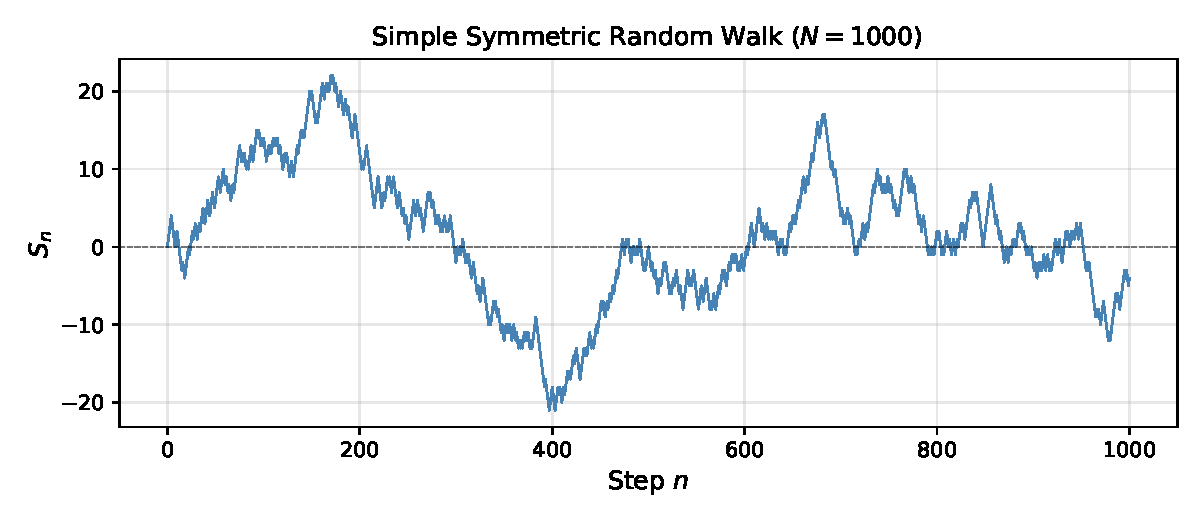
\includegraphics[width=0.82\textwidth]{fig_ssrw_single}
  \end{center}
  \textit{A single realisation of the SSRW for $N = 1000$ steps.  The walk
  exhibits long ``excursions'' (extended periods) on one side of zero ---
  a direct consequence of the arcsine law discussed in Section 1.2.3.}

\end{frame}

%% ------------------------------------------------------------------
\begin{frame}[allowframebreaks]{1.2.2 How Large Are the Fluctuations? The Law of the Iterated Logarithm}

  Our first quantitative question is: how large does $|S_n|$ (the absolute
  value of the walk position, measuring how far from zero the player A's
  fortune has gone) grow as $n$ (the number of steps) increases?  To answer
  this, we try normalising the walk by different functions of $n$ and ask
  what the normalised sequence converges to.

  \textbf{Three candidate normalisation rates.}  Since $|S_n| \le n$ always,
  we can normalise by any function of $n$ that is between 1 and $n$.  There
  are three natural candidates, each giving a different type of answer.

  \begin{itemize}
    \item \textbf{Normalise by $n$:} The Strong Law of Large Numbers (SLLN)
      gives $S_n/n \to 0$ almost surely (with probability 1) as $n \to \infty$.
      This is because the mean (expected value) of each step $X_j$ is zero:
      $\mathbb{E}[X_j] = (+1)(1/2) + (-1)(1/2) = 0$.  So dividing by $n$ is
      \emph{too aggressive} --- the normalised walk collapses to zero and we
      learn nothing about the actual fluctuations.

    \item \textbf{Normalise by $\sqrt{n}$ (square root of $n$):}  The Central
      Limit Theorem (CLT) says $S_n / \sqrt{n}$ converges \emph{in
      distribution} to $\mathcal{N}(0,1)$ (the standard normal distribution,
      also called the bell curve).  Here $\mathcal{N}(0,1)$ (N zero one) has
      mean 0 and variance 1.  However, the sequence $S_n/\sqrt{n}$ does
      \emph{not} converge almost surely --- it oscillates indefinitely between
      large positive and large negative values.  So $\sqrt{n}$ is
      \emph{too weak}: the normalised walk does not settle.

    \item \textbf{Normalise by $\sqrt{2n \log \log n}$:}  This is the
      \emph{correct} scale, as stated by the Law of the Iterated Logarithm.
      Here ``$\log$'' (log) denotes the natural logarithm (base $e$, where
      $e \approx 2.71828$), and ``$\log \log n$'' means the logarithm of the
      logarithm of $n$ --- an extremely slowly growing function of $n$.
      The factor ``iterated logarithm'' in the name refers to this double
      application of the logarithm.
  \end{itemize}

  \begin{block}{Law of the Iterated Logarithm (LIL) --- Khintchine, 1924; Kolmogorov, 1929}
    For the simple symmetric random walk $S_n = \sum_{j=1}^n X_j$, where each
    $X_j \in \{-1, +1\}$ with probability $1/2$ each, the following hold with
    probability 1:
    \[
      \mathbb{P}\!\left(
        \limsup_{n \to \infty}
        \frac{S_n}{\sqrt{2n \log \log n}} = +1
      \right) = 1
      \quad\text{and}\quad
      \mathbb{P}\!\left(
        \liminf_{n \to \infty}
        \frac{S_n}{\sqrt{2n \log \log n}} = -1
      \right) = 1.
    \]
  \end{block}

  Here ``$\limsup_{n \to \infty}$'' (limit superior, read ``lim-sup as $n$
  goes to infinity'') is the largest value that the sequence gets close to
  infinitely often as $n$ grows --- intuitively, the highest ``ceiling'' the
  sequence keeps touching without permanently exceeding.  Symmetrically,
  ``$\liminf_{n \to \infty}$'' (limit inferior, or ``lim-inf'') is the
  smallest such accumulation point, the lowest floor the sequence keeps
  touching.  The two formulas together say: with probability 1, the
  walk reaches arbitrarily close to $+\sqrt{2n \log \log n}$ infinitely often,
  and reaches arbitrarily close to $-\sqrt{2n \log \log n}$ infinitely often,
  but never permanently exceeds either boundary.

  \begin{alertblock}{How to Read the LIL}
    In plain language: the walk $S_n$ never settles down --- it oscillates
    without bound.  But it stays within a well-defined almost-sure
    \emph{envelope}: $|S_n| \le \sqrt{2n \log \log n}$ for all sufficiently
    large $n$, with probability 1.  The walk touches the upper boundary
    $+\sqrt{2n \log \log n}$ infinitely often, and likewise touches the lower
    boundary $-\sqrt{2n \log \log n}$ infinitely often.  The ``iterated
    logarithm'' $\log \log n$ is a tiny correction factor: it grows
    incredibly slowly (for $n = 10^{100}$, we have $\log \log n \approx 5.4$),
    so the envelope is only slightly wider than the naive $\sqrt{n}$ envelope.
    This precise scaling is not merely a theoretical curiosity --- it has
    practical consequences for how long you need to run a simulation before
    results stabilise.
  \end{alertblock}

  \framebreak

  \textbf{Concrete numerical illustration of $\sqrt{2n \log \log n}$.}

  Let us plug in specific values to get a feel for how this envelope grows.
  For $n = 10{,}000$ (ten thousand steps):

  \begin{exampleblock}{Worked Numerical Calculation at $n = 10{,}000$}
    \begin{align*}
      \sqrt{n} &= \sqrt{10{,}000} = 100, \\[4pt]
      \log n &= \log(10{,}000) = \log(10^4) = 4\log(10) \approx 4 \times 2.303 \approx 9.21
        \quad\text{(natural log)}, \\[4pt]
      \log \log n &= \log(9.21) \approx 2.22, \\[4pt]
      \sqrt{2n \log \log n} &= \sqrt{2 \times 10{,}000 \times 2.22}
        = \sqrt{44{,}400} \approx 211.
    \end{align*}
    So the LIL envelope at step $n = 10{,}000$ is approximately $\pm 211$,
    which is about $2.11$ times larger than the ``naive'' square-root
    boundary of $\pm\sqrt{n} = \pm 100$.  The gap between the two
    envelopes widens only very slowly (logarithmically) as $n$ grows further.
  \end{exampleblock}

  \begin{columns}[T]
    \begin{column}{0.52\textwidth}
      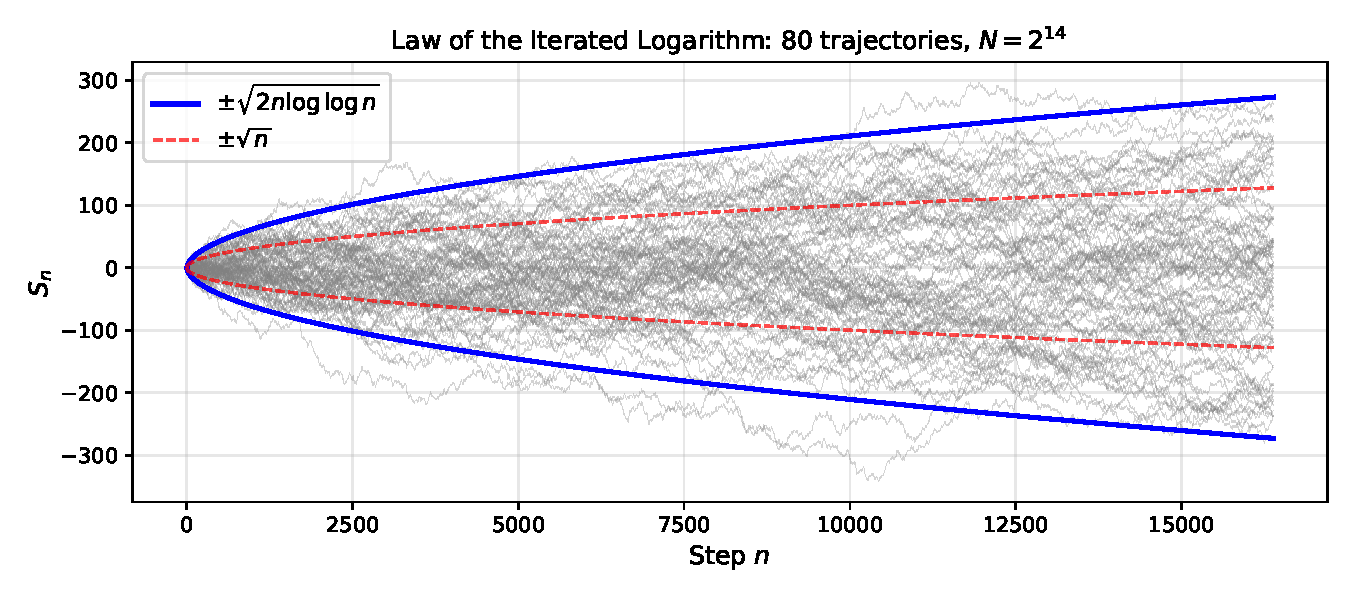
\includegraphics[width=\textwidth]{fig_lil_envelope}
    \end{column}
    \begin{column}{0.45\textwidth}
      \textbf{Simulation evidence.}  The figure shows 80 independent SSRW
      trajectories of length $n = 2^{14} = 16{,}384$ steps, each started at
      $S_0 = 0$.  The solid blue curves are the LIL envelopes
      $\pm\sqrt{2n \log \log n}$; the red dashed lines are $\pm\sqrt{n}$ for
      comparison.  Every simulated path stays inside the LIL envelope,
      consistent with the theorem.  Several paths are seen to brush against
      the LIL envelope --- this is also consistent with the theorem, which
      says the envelope is touched infinitely often in the limit.
    \end{column}
  \end{columns}

  \begin{alertblock}{Key Takeaway: The Correct Scale of Fluctuations}
    The walk grows neither as slowly as $\sqrt{n}$ nor as fast as $n$.  The
    precise almost-sure scale is $\sqrt{2n \log \log n}$, which is only
    slightly (logarithmically) larger than $\sqrt{n}$.  This precise scaling
    has important practical consequences: it tells you how far from the mean
    a simulation output can stray if you run it for $n$ steps, which informs
    decisions about how long to run a simulation and how to interpret
    unexpected extreme outputs.
  \end{alertblock}

\end{frame}

%% ------------------------------------------------------------------
\begin{frame}[allowframebreaks]{1.2.3 The Arcsine Law}

  The arcsine law provides exact answers to questions Q1 and Q2, and stands
  as one of the most counter-intuitive results in elementary probability theory.
  Understanding it thoroughly will permanently change how you think about
  ``fairness'' in random processes.

  \textbf{What intuition suggests --- and why it is wrong.}  Since the walk is
  perfectly symmetric (the probability of going up equals the probability of
  going down at every step), you might expect the fraction of time that player
  A is winning to be typically close to $1/2$.  After all, the game is fair:
  shouldn't both players lead for roughly equal portions of the time?  The
  arcsine law gives the precise, surprising answer: being ahead for
  \emph{nearly all} of the time or \emph{nearly none} of the time is
  \emph{most likely}, while being ahead for exactly half the time is the
  \emph{least likely} outcome of all.

  \begin{block}{Arcsine Law (Feller, 1950; Durrett, 1996)}
    For $0 \le \alpha < \beta \le 1$ (where $\alpha$ (alpha) and $\beta$
    (beta) are fractions between 0 and 1 representing lower and upper bounds
    on the fraction of time player A leads), as $n \to \infty$ (as the number
    of steps grows without bound), the fraction of time spent above zero
    converges in distribution:
    \[
      \mathbb{P}\!\left(
        \alpha \;\le\; \frac{L^+_{2n}}{2n} \;\le\; \beta
      \right)
      \;\longrightarrow\;
      \int_\alpha^\beta \frac{dx}{\pi \sqrt{x(1-x)}}.
      \tag{1.2.1}
    \]
  \end{block}

  \begin{block}{Notation for the Arcsine Law Formula}
    In this formula:
    \begin{itemize}
      \item $\mathbb{P}(\cdot)$ (blackboard P) is the probability of the
        event described.
      \item $L^+_{2n}$ (L-plus subscript 2n) counts the number of steps during
        which player A is winning.
      \item $L^+_{2n}/(2n)$ is the \emph{fraction} of the total $2n$ steps
        during which player A leads, a number between 0 and 1.
      \item $\alpha$ (alpha) and $\beta$ (beta) are two fractions with
        $0 \le \alpha < \beta \le 1$.
      \item $\int_\alpha^\beta$ (integral from $\alpha$ to $\beta$) computes
        the area under the curve $1/(\pi\sqrt{x(1-x)})$ between $x = \alpha$
        and $x = \beta$.
      \item $\pi$ (pi) is the mathematical constant $\approx 3.14159$.
      \item $x(1-x)$ (x times one minus x) is zero at both endpoints $x=0$
        and $x=1$, so the density $1/(\pi\sqrt{x(1-x)})$ is infinitely large
        there.
    \end{itemize}
  \end{block}

  \framebreak

  \textbf{Why is it called the ``arcsine'' law?}  The cumulative distribution
  function of the limiting distribution (the probability that the fraction of
  winning time is at most $\beta$) can be computed in closed form by evaluating
  the integral:
  \[
    \int_0^\beta \frac{dx}{\pi\sqrt{x(1-x)}}
    \;=\; \frac{2}{\pi}\arcsin\!\bigl(\sqrt{\beta}\bigr),
  \]
  where $\arcsin$ (arcsine, the inverse of the sine function) appears
  explicitly.  This closed form is where the distribution gets its name.

  The corresponding probability density function (PDF) is:
  \[
    p(x) = \frac{1}{\pi\sqrt{x(1-x)}}, \qquad 0 < x < 1.
  \]
  This density has a characteristic \textbf{U-shape}: it equals $+\infty$
  at $x = 0$ and at $x = 1$ (so the walk is most likely to spend all its
  time on one side of zero, or none of its time there), and achieves its
  minimum value of $2/\pi \approx 0.637$ at $x = 1/2$ (the least likely
  outcome is a perfectly equal split of the lead).  The U-shape is the
  mathematical signature of the gambler's fallacy: extreme outcomes are
  more common than moderate ones.

  \begin{exampleblock}{Worked Numerical Calculation: Probability of a ``Fair'' vs.\ ``Extreme'' Outcome}
    The probability that player A leads between 40\% and 60\% of the time
    (a ``near-equal'' split):
    \[
      \mathbb{P}\!\left(0.4 \le \tfrac{L^+_{2n}}{2n} \le 0.6\right)
      \approx \tfrac{2}{\pi}\arcsin(\sqrt{0.6}) - \tfrac{2}{\pi}\arcsin(\sqrt{0.4})
      \approx 0.795 - 0.667 \approx 0.128.
    \]
    Only about $12.8\%$ of long games end with a near-equal split of the lead!

    The probability of an ``extreme'' outcome (one player leads more than 90\%
    of the time):
    \[
      \mathbb{P}\!\left(\tfrac{L^+_{2n}}{2n} \le 0.1\right)
      + \mathbb{P}\!\left(\tfrac{L^+_{2n}}{2n} \ge 0.9\right)
      \approx 2 \times \tfrac{2}{\pi}\arcsin(\sqrt{0.1})
      \approx 2 \times 0.205 \approx 0.410.
    \]
    Over $41\%$ of games end with one player dominating for more than $90\%$
    of the time --- more than three times as common as the near-equal split!
    This is the arcsine law in action.
  \end{exampleblock}

  \framebreak

  \begin{center}
    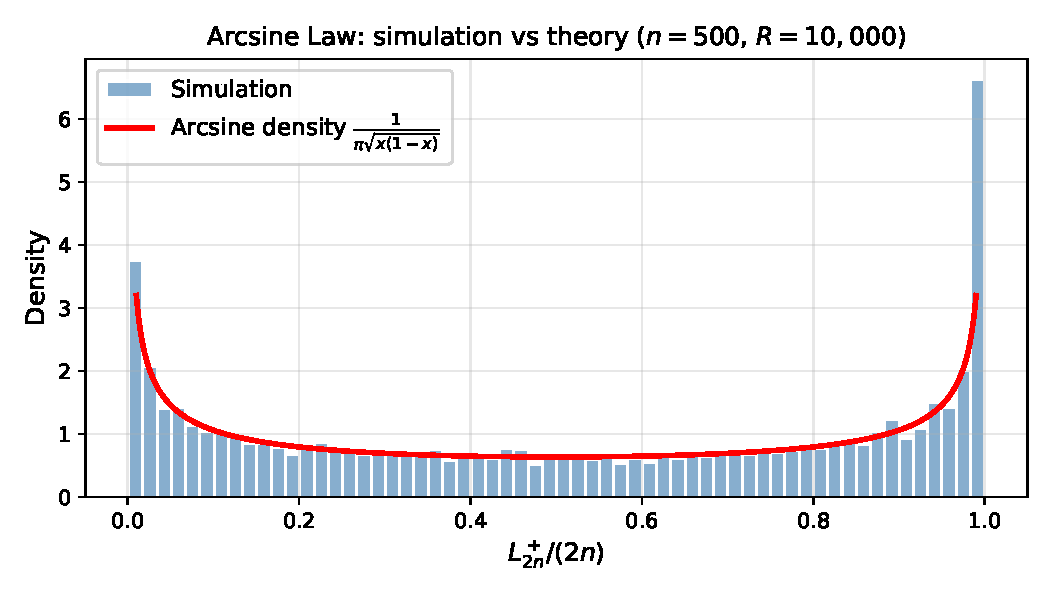
\includegraphics[width=0.60\textwidth]{fig_arcsine_law}
  \end{center}
  \textit{Histogram of $L^+_{1000}/1000$ (fraction of 1000-step walks spent
  above zero) from $R = 10{,}000$ independent replications.  The red curve is
  the theoretical arcsine density $p(x) = 1/(\pi\sqrt{x(1-x)})$.  The
  U-shape is clearly visible: the bars at both extremes (near 0 and near 1)
  are tallest, while the bar near $x = 1/2$ is shortest.  The simulation
  matches the theory closely.}

  \begin{alertblock}{Key Insight: The Gambler's Fallacy Refuted}
    The arcsine law overturns the naive intuition that ``fair'' games lead to
    equal sharing of the lead.  A player who is behind for the first 99\% of
    a game is \emph{not} especially likely to ``recover'' and take the lead
    before the end.  In fact, being behind (or ahead) for the entire game is
    a completely typical and mathematically expected outcome.  This is the
    \emph{gambler's fallacy} refuted: past losses do not make future wins more
    likely in a symmetric game, because the walk has no memory.  Each coin
    toss is independent of all previous ones.
  \end{alertblock}

  \textbf{Connection to randomness testing.}  The arcsine law is not merely
  a theoretical curiosity about gambling.  In Section~2.5, we will use the
  arcsine law to construct a \emph{statistical test} for the quality of a
  pseudorandom number generator: if the generator truly produces random
  numbers, then the statistic $L^+_{2n}/(2n)$ computed from its output should
  follow the arcsine distribution.  A significant deviation from the arcsine
  distribution signals a defect or pattern in the generator.

\end{frame}

%% ------------------------------------------------------------------
\begin{frame}[fragile]{1.2.4 Python: Simulating the SSRW and the LIL Envelope}

  The following code simulates a single SSRW trajectory and overlays the
  LIL envelope $\pm\sqrt{2n \log \log n}$ to visually verify the theorem.
  The key implementation step is converting uniform integers in $\{0, 1\}$
  to steps in $\{-1, +1\}$ via the formula $X_j = 1 - 2B_j$ where
  $B_j \in \{0, 1\}$: when $B_j = 0$ we get $X_j = 1$ (heads), and when
  $B_j = 1$ we get $X_j = -1$ (tails).  The function \texttt{np.cumsum}
  (short for ``cumulative sum'') then computes all partial sums $S_1, S_2,
  \ldots, S_{2N}$ at once as an array, without any explicit loop.

\begin{lstlisting}[style=python]
import numpy as np
import matplotlib.pyplot as plt
from numpy.random import default_rng

rng = default_rng(seed=31415)
N   = 1000                               # walk has 2N steps

steps = 1 - 2 * rng.integers(0, 2, size=2*N)  # {-1, +1}
S     = np.concatenate([[0], steps.cumsum()])  # S_0=0, S_1,...,S_{2N}

# LIL envelope: +/- sqrt(2 * n * log(log(n)))
# We start from n=2 to avoid log(log(1))=log(0) which is -infinity
n_arr    = np.arange(2, 2*N + 1)
envelope = np.sqrt(2 * n_arr * np.log(np.log(n_arr)))

fig, ax = plt.subplots(figsize=(10, 3.5))
ax.plot(range(2*N + 1), S, lw=0.8, color='steelblue', label='$S_n$')
ax.plot(n_arr,  envelope, 'b-', lw=1.8, alpha=0.7,
        label=r'LIL: $\pm\sqrt{2n\log\log n}$')
ax.plot(n_arr, -envelope, 'b-', lw=1.8, alpha=0.7)
ax.axhline(0, color='k', lw=0.5, ls='--')
ax.set_xlabel('Step $n$')
ax.set_ylabel('$S_n$')
ax.legend(loc='upper left')
ax.grid(True, alpha=0.3)
plt.tight_layout()
plt.show()
\end{lstlisting}

\end{frame}

%% ------------------------------------------------------------------
\begin{frame}[fragile]{1.2.5 Python: Verifying the Arcsine Law}

  To verify the arcsine law statistically, we simulate $R = 10{,}000$
  independent walks of $2n = 1000$ steps each, compute $L^+_{2n}/(2n)$ for
  each walk, and compare the empirical histogram to the theoretical arcsine
  density.  Vectorising the simulation over all $R$ replications simultaneously
  using NumPy's array operations (operating on the entire matrix at once rather
  than looping over replications) makes this fast enough to run interactively
  on a laptop in a few seconds.

\begin{lstlisting}[style=python]
import numpy as np
import matplotlib.pyplot as plt
from numpy.random import default_rng

def fraction_above_zero(n=500, R=10_000, seed=0):
    """Return array of L^+_{2n}/(2n) for R independent walks.

    n  : half-length (walk has 2n steps)
    R  : number of independent replications
    Returns: array of shape (R,), each value in [0,1]
    """
    rng   = default_rng(seed)
    # shape: (R, 2n) -- each row is one walk's steps
    steps = 1 - 2 * rng.integers(0, 2, size=(R, 2*n))
    # cumsum along axis=1, prepend column of zeros --> shape (R, 2n+1)
    S = np.hstack([np.zeros((R, 1)), steps.cumsum(axis=1)])
    # Step j is counted if S_{j-1}>=0 OR S_j>=0 (at least one endpoint >= 0)
    above = (S[:, :-1] >= 0) | (S[:, 1:] >= 0)
    return above.sum(axis=1) / (2*n)   # shape (R,), each in [0,1]

fracs = fraction_above_zero(n=500, R=10_000)

# Theoretical arcsine density: f(x) = 1 / (pi * sqrt(x*(1-x)))
x   = np.linspace(0.005, 0.995, 500)
pdf = 1.0 / (np.pi * np.sqrt(x * (1.0 - x)))

plt.figure(figsize=(7, 4))
plt.hist(fracs, bins=60, density=True, alpha=0.6, color='steelblue',
         label='Simulation ($n=500$, $R=10000$)')
plt.plot(x, pdf, 'r-', lw=2.2,
         label=r'Arcsine density $\frac{1}{\pi\sqrt{x(1-x)}}$')
plt.xlabel(r'$L^+_{2n}/(2n)$  (fraction of time player A is winning)')
plt.ylabel('Density')
plt.title('Arcsine Law: verified by simulation')
plt.legend()
plt.tight_layout()
plt.show()
\end{lstlisting}

\end{frame}

%% ===================================================================
\section{1.3 Travelling Salesman Problem}
%% ===================================================================

\begin{frame}[allowframebreaks]{1.3.1 The TSP: Problem Statement and Why It Is Hard}

  The Travelling Salesman Problem (TSP) is a paradigmatic hard combinatorial
  optimisation problem.  It arises in many real-world contexts: logistics
  (planning delivery routes for trucks), circuit board manufacturing
  (minimising the travel distance of a drilling machine), genome sequencing
  (ordering DNA fragments along a chromosome), and telescope scheduling
  (minimising slew time between observations).  It is our second motivating
  example for Monte Carlo methods, because it illustrates why randomised
  heuristics are indispensable when exact search is computationally infeasible.

  \textbf{The problem.}  A salesman must visit $n$ cities exactly once and
  return to the starting city, forming a closed tour.  The distance (or cost)
  of travelling from city $i$ to city $j$ is given by the entry $\mathbf{M}_{ij}$
  (bold M subscript ij, read ``M sub i j'', a real number representing the
  travel cost) in an $n \times n$ matrix $\mathbf{M}$ (bold M, an
  $n$-by-$n$ array of all pairwise distances).  The entry is
  $\mathbf{M}_{ij} = \infty$ (infinity) if there is no direct route from
  city $i$ to city $j$.  The goal is to find the \emph{shortest closed tour}
  --- a route that starts and ends at the same city and visits each city
  exactly once, with the smallest total travel distance.

  Mathematically, a \emph{tour} is a permutation $\sigma$ (sigma (sig-ma), a
  re-ordering or rearrangement) of the cities $\{1, \ldots, n\}$.  The
  expression $\sigma(k)$ (sigma of k) denotes the $k$-th city visited.
  The total length (total distance) of the tour is:
  \[
    l(\sigma) = \sum_{k=1}^{n-1} \mathbf{M}_{\sigma(k),\,\sigma(k+1)}
    + \mathbf{M}_{\sigma(n),\,\sigma(1)}.
  \]
  The sum $\sum_{k=1}^{n-1}$ (sigma from $k$ equals 1 to $n-1$) adds up the
  distances of all consecutive legs of the tour except the final return leg;
  the last term $\mathbf{M}_{\sigma(n),\sigma(1)}$ adds the distance from the
  last city back to the first, closing the loop.

  \begin{block}{Optimisation Problem: Find the Shortest Tour}
    We seek the optimal permutation (the ordering of cities that gives the
    shortest total distance):
    \[
      \sigma^* = \operatorname*{arg\,min}_{\sigma \in S_n} l(\sigma),
    \]
    where $S_n$ (S subscript n) denotes the set of all $n!$ permutations of
    the $n$ cities, and ``$\operatorname{arg\,min}$'' (argument of the minimum)
    means ``the permutation $\sigma$ for which $l(\sigma)$ achieves the
    minimum value.''  The symbol $\sigma^*$ (sigma-star) conventionally denotes
    the optimal solution.
  \end{block}

  \framebreak

  \textbf{Why is the TSP computationally hard?}  The search space $S_n$
  contains $n!$ (n factorial, meaning $1 \times 2 \times 3 \times \cdots
  \times n$) possible tours.  The factorial function grows faster than any
  fixed exponential, as the following table dramatically illustrates:

  \begin{center}
  \begin{tabular}{rlr}
    \toprule
    $n$ cities & $n!$ permutations & Time to check all at $10^9$/sec \\
    \midrule
    10  & $3{,}628{,}800 \approx 3.6 \times 10^6$  & $0.004$ seconds \\
    15  & $\approx 1.3 \times 10^{12}$  & $21$ minutes \\
    20  & $\approx 2.4 \times 10^{18}$  & $76$ years \\
    50  & $\approx 3.0 \times 10^{64}$  & longer than the age of the universe \\
    \bottomrule
  \end{tabular}
  \end{center}

  At $10^9$ (one billion) tour evaluations per second, evaluating all $50!$
  tours would require approximately $10^{55}$ years.  The current age of the
  universe is only about $1.4 \times 10^{10}$ years.  Exhaustive search is
  not just slow --- it is completely and permanently infeasible for $n \ge 25$
  or so, regardless of how fast computers become.

  The TSP belongs to the class of \textbf{NP-complete} problems: no algorithm
  is known that solves all instances in polynomial time (time proportional to
  some fixed power $n^k$), and the overwhelming consensus among theoretical
  computer scientists is that no such algorithm exists.  Exact algorithms using
  clever branch-and-bound methods are practical only for $n \lesssim 50$ (and
  can take hours even then).

  \framebreak

  \textbf{Monte Carlo heuristics for the TSP.}  Since exact optimisation is
  infeasible for large $n$, we use \emph{randomised approximation algorithms}
  that efficiently find near-optimal (but not necessarily exactly optimal)
  solutions.

  \begin{description}
    \item[Random restart.]  Sample $R$ (integer $R$, the number of trials)
      random permutations uniformly from $S_n$, evaluate $l(\sigma)$ for each,
      and return the best one found.  This is the simplest Monte Carlo approach,
      analogous to drawing lottery tickets and keeping the best.  For $n = 15$
      cities and $R = 20{,}000$ trials, random search typically finds a tour
      that is 30--50\% longer than the optimal tour.

    \item[Simulated Annealing (Ch.~7).]  Start with a random tour.  At each
      step, propose a small local modification called a \emph{2-opt move}:
      remove two edges from the tour and reconnect the four endpoints
      differently, reversing the segment between them.  Always accept
      improvements.  Accept worsening moves with probability
      $\exp(-\Delta l / T)$ (read ``exponential of minus delta-l over T''),
      where $\Delta l$ (delta l, the Greek letter delta meaning ``change in'')
      is the increase in tour length due to the move, and $T$ (T) is a
      ``temperature'' parameter that decreases slowly over time.  Accepting
      worsening moves with some probability allows escape from local optima.
      This is the key insight behind simulated annealing.

    \item[Cross-Entropy Method (Chs.~5, 7).]  Maintain a probability
      distribution over tours, sample batches of tours from it, keep the best
      fraction (the ``elite sample''), and update the distribution to assign
      higher probability to elite tours.  Repeating this cycle drives the
      distribution toward near-optimal tours.
  \end{description}

  \begin{center}
    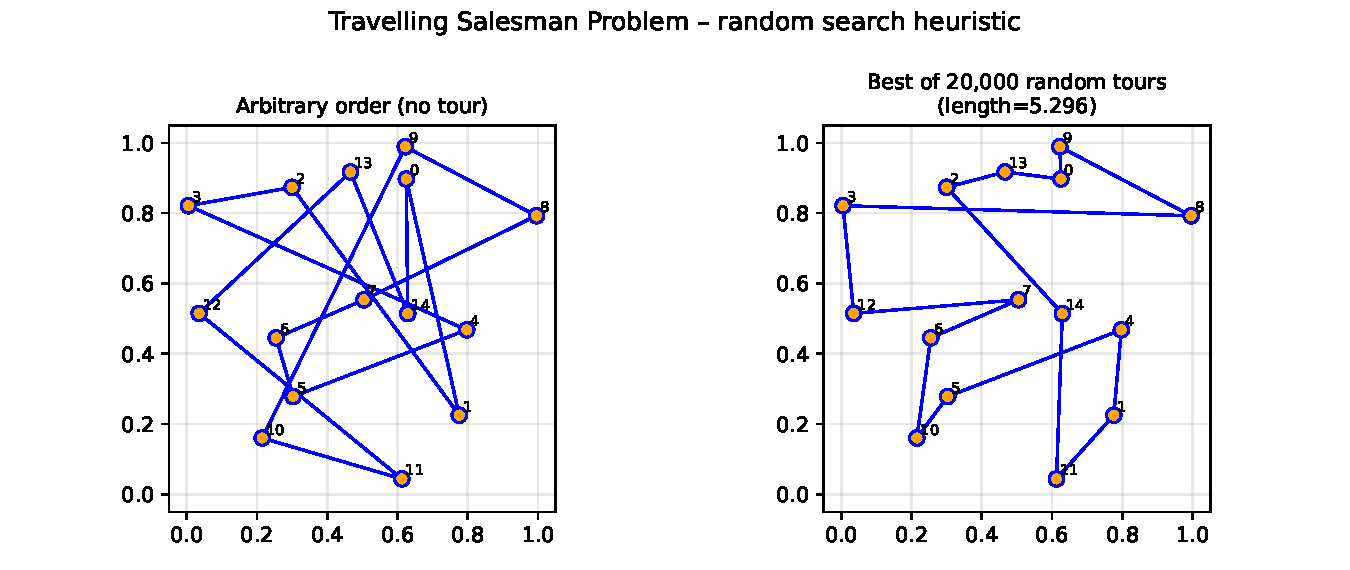
\includegraphics[width=0.80\textwidth]{fig_tsp}
  \end{center}
  \textit{Left: 15 random cities connected in an arbitrary random order (no
  optimisation; many edge crossings visible, which is always suboptimal).
  Right: best tour found by random search over $R = 20{,}000$ random
  permutations.  The absence of crossings is a necessary (but not sufficient)
  condition for an optimal tour.}

\end{frame}

%% ------------------------------------------------------------------
\begin{frame}[fragile]{1.3.2 Python: Random Tour Search for the TSP}

  The following implementation evaluates $R = 20{,}000$ random tours of
  $n = 15$ cities placed uniformly at random in the unit square $[0,1]^2$,
  and keeps the shortest tour found.  The function \texttt{tour\_length}
  uses \texttt{np.roll} (shift all elements of the array by one position,
  wrapping the last element to the front) to implement the cyclic distance
  computation efficiently without an explicit loop over cities.

\begin{lstlisting}[style=python]
import numpy as np
from numpy.random import default_rng

def tour_length(cities, perm):
    """Compute the total Euclidean length of a closed tour.

    cities : shape (n, 2) -- the (x, y) coordinates of each city
    perm   : permutation of {0, ..., n-1} -- the order to visit cities
    Returns: the total distance of the tour (a single float)
    """
    # shifted[k] = perm[k+1 mod n], so it gives the NEXT city after perm[k]
    # This creates the "closing the loop" effect automatically
    shifted = np.roll(perm, -1)
    # Compute (x, y) differences for each leg of the tour: shape (n, 2)
    diffs   = cities[perm] - cities[shifted]
    # Euclidean distance of each leg: sqrt(dx^2 + dy^2), then sum all legs
    return np.linalg.norm(diffs, axis=1).sum()

def random_tour_search(cities, R=20_000, seed=42):
    """Return (best_tour, best_length) from R random permutations.

    R    : number of random tours to try (more is better but slower)
    seed : random seed for reproducibility
    """
    rng = default_rng(seed)
    n   = len(cities)
    best_len, best_tour = np.inf, None
    for _ in range(R):
        perm = rng.permutation(n)          # draw a uniform random tour
        L    = tour_length(cities, perm)
        if L < best_len:                   # keep the best found so far
            best_len  = L
            best_tour = perm.copy()
    return best_tour, best_len

# Generate 15 random cities uniformly in the unit square [0,1]^2
rng    = default_rng(seed=7)
cities = rng.random((15, 2))

tour, length = random_tour_search(cities, R=20_000)
print(f"Best tour length (random search, R=20000): {length:.4f}")
# Simulated annealing (Chapter 7) achieves roughly 30% shorter tours
\end{lstlisting}

  This simple baseline is instructive: evaluating $R = 20{,}000$ random tours
  is entirely feasible on a modern laptop (completing in milliseconds), yet
  the result is typically far from the optimal tour.  Chapter~7 develops
  simulated annealing, which finds near-optimal solutions in comparable
  computational time by intelligently exploring the neighbourhood of the
  current tour rather than jumping to entirely random permutations each time.

\end{frame}

%% ===================================================================
\section{1.4 Computing Integrals with Monte Carlo}
%% ===================================================================

\begin{frame}[allowframebreaks]{1.4.1 The Monte Carlo Integration Framework}

  One of the most important and widely used applications of Monte Carlo methods
  is numerical estimation of integrals, particularly in high dimensions where
  classical deterministic quadrature methods become hopelessly expensive.  This
  section develops the basic theory and shows why MC is \emph{completely
  dimension-independent} in its convergence rate --- a remarkable property
  that no grid-based quadrature method can match.

  \textbf{The integration problem.}  We want to compute the integral:
  \[
    I = \int_{[0,1]^d} k(\mathbf{u})\, d\mathbf{u},
  \]

  \begin{block}{Notation for the Integration Problem}
    In this formula:
    \begin{itemize}
      \item $k : [0,1]^d \to \mathbb{R}$ ($k$, a function) maps each point in
        the $d$-dimensional unit hypercube to a real number.  This is the
        function whose integral we want.
      \item $[0,1]^d$ (the $d$-dimensional unit hypercube) is the set of all
        $d$-dimensional vectors $\mathbf{u} = (u_1, \ldots, u_d)$ where each
        coordinate $u_i$ lies between 0 and 1.
      \item $d$ (the dimension) is the number of coordinates, which can be
        very large (e.g., $d = 100$ or $d = 1000$).
      \item $\mathbf{u}$ (bold u) is the variable of integration, a
        $d$-dimensional vector.
      \item $d\mathbf{u}$ denotes integration with respect to all $d$ coordinates
        simultaneously.
    \end{itemize}
    This formulation covers a large class of problems: any integral over a
    bounded domain can be transformed to this form by a change of variables.
  \end{block}

  \textbf{The probabilistic interpretation.}  If $\mathbf{U}$ (bold U, a
  random vector) is uniformly distributed on $[0,1]^d$ (meaning each coordinate
  is independently and uniformly distributed on $[0,1)$), then the integral
  equals the expected value:
  \[
    I \;=\; \mathbb{E}[k(\mathbf{U})].
  \]
  This identity --- the integral equals the expected value of $k$ at a uniform
  random point --- is the fundamental bridge between integration and probability
  that makes Monte Carlo work.  It tells us: to estimate an integral, draw
  random points uniformly and average the function values.

  \begin{block}{Monte Carlo Estimator}
    Let $\mathbf{U}_1, \mathbf{U}_2, \ldots, \mathbf{U}_n$ be i.i.d.\
    (independent and identically distributed) uniform random vectors on
    $[0,1]^d$, where $n$ is the number of samples.  Define the
    \textbf{Monte Carlo estimator}:
    \[
      \hat{Y}_n = \frac{1}{n} \sum_{i=1}^{n} k(\mathbf{U}_i).
      \tag{1.2.2}
    \]
    Here $\hat{Y}_n$ (Y-hat subscript n; the hat $\hat{\phantom{Y}}$ means
    ``estimate'' or ``approximation'') is the sample average of $n$ independent
    evaluations of $k$.  The index $i$ runs from 1 to $n$, and the sum
    $\sum_{i=1}^n$ (Sigma from $i$ equals 1 to $n$) adds all $n$ values.
    By the Strong Law of Large Numbers (SLLN), $\hat{Y}_n \to I$ almost
    surely (with probability 1) as $n \to \infty$.  The estimator is
    \textbf{unbiased}: $\mathbb{E}[\hat{Y}_n] = I$ for every $n$, meaning
    it is correct on average for any number of samples.
  \end{block}

  \framebreak

  \begin{block}{Variance and Error Rate of the MC Estimator}
    Since the $\mathbf{U}_i$ are i.i.d., the variance (the squared spread
    around the mean) of $\hat{Y}_n$ is:
    \[
      \mathrm{Var}(\hat{Y}_n) = \frac{\sigma^2}{n},
      \quad\text{where}\quad
      \sigma^2 = \mathrm{Var}(k(\mathbf{U}))
      = \int_{[0,1]^d} k(\mathbf{u})^2\, d\mathbf{u} - I^2.
    \]
    Here $\sigma^2$ (sigma-squared, where $\sigma$ (sigma) is the Greek
    letter for ``s'') is the variance of a single evaluation $k(\mathbf{U})$,
    measuring how spread out single evaluations are around the true integral
    $I$.  The quantity $\sigma$ (sigma) is the standard deviation: it
    measures the typical deviation of one evaluation from the mean, in the
    same units as $k$.  By the Central Limit Theorem (CLT), for large $n$:
    \[
      \sqrt{n}\,(\hat{Y}_n - I) \;\xrightarrow{d}\; \mathcal{N}(0, \sigma^2),
    \]
    meaning $\sqrt{n}$ (square root of $n$) times the error converges
    \emph{in distribution} (symbolised by $\xrightarrow{d}$) to a normal
    (bell-curve) distribution with mean 0 and variance $\sigma^2$.
    The root-mean-squared error (RMSE) of the estimator is:
    \[
      \mathrm{RMSE}(\hat{Y}_n)
      \;=\; \sqrt{\mathbb{E}\bigl[(\hat{Y}_n - I)^2\bigr]}
      \;=\; \frac{\sigma}{\sqrt{n}}
      \;=\; O(n^{-1/2}).
    \]
    Here RMSE (root mean squared error) is the standard measure of estimation
    accuracy --- the square root of the average squared difference between the
    estimate and the truth.  The notation $O(n^{-1/2})$ (``big-O of $n$ to
    the minus one-half'') means the error decreases at the rate $1/\sqrt{n}$
    as $n$ grows.
  \end{block}

  \begin{alertblock}{How to Read This Error Rate}
    The RMSE is $\sigma/\sqrt{n}$: to halve the error, you must
    \emph{quadruple} the number of samples (because $1/\sqrt{4n} = (1/2)
    \cdot 1/\sqrt{n}$, so multiplying $n$ by 4 divides the RMSE by 2).
    This is a ``diminishing returns'' relationship: going from $n = 100$ to
    $n = 400$ halves the error; going from $n = 400$ to $n = 1{,}600$ halves
    it again.  The critically important fact is that this rate $O(n^{-1/2})$
    is \textbf{completely independent of the dimension $d$} --- whether $d = 1$
    or $d = 100$, you need the same number of samples to achieve the same RMSE.
    This dimension-independence is the defining advantage of Monte Carlo.
  \end{alertblock}

  \framebreak

  \textbf{The curse of dimensionality and why Monte Carlo wins.}

  A regular grid with $m$ (integer $m$) points per dimension requires $m^d$
  (m to the power d) total function evaluations.  This number grows
  exponentially with the dimension $d$.  A standard trapezoidal quadrature
  rule on this grid achieves error $O(m^{-2/d})$: to achieve error
  $\varepsilon$ (epsilon, a small positive target accuracy), you need
  $m \sim \varepsilon^{-d/2}$ points per dimension and $m^d \sim
  \varepsilon^{-d}$ total evaluations.

  \begin{center}
  \begin{tabular}{lcc}
    \toprule
    Method & Error & Evaluations for $\varepsilon = 10^{-2}$, $d = 10$ \\
    \midrule
    Regular grid ($m^d$ pts)   & $O(m^{-2/d})$ & $100^{10} = 10^{20}$ \\
    Monte Carlo ($n$ pts)      & $O(n^{-1/2})$ & $\sigma^2 / \varepsilon^2 \approx 10^4$ \\
    \bottomrule
  \end{tabular}
  \end{center}

  For $d = 10$ dimensions and target error $\varepsilon = 0.01$, the grid
  requires $10^{20}$ function evaluations (computationally impossible), while
  MC requires only about $10^4$ evaluations (completing in milliseconds on a
  laptop).  For $d \ge 5$, Monte Carlo almost always dominates grid-based
  quadrature, and the advantage grows exponentially with each additional
  dimension.

  \framebreak

  \textbf{Discrepancy: measuring how uniformly points fill the space.}

  The concept of \emph{discrepancy} provides another perspective on the MC
  error rate, and connects the quality of a point set (how uniformly it
  covers the space) to the integration error it produces.

  \begin{block}{Discrepancy (formula 1.2.3 in the book)}
    Given a sequence of points $\mathbf{x}_1, \ldots, \mathbf{x}_n \in
    [0,1)^d$, the \emph{star-discrepancy} $D^*$ (D-star) measures how far
    the empirical distribution of those points is from perfect uniformity:
    \[
      D(\mathbf{x}_1, \ldots, \mathbf{x}_n;\, \mathcal{B})
      = \sup_{A \in \mathcal{B}}
        \left|
          \frac{\#\{1 \le i \le n : \mathbf{x}_i \in A\}}{n}
          - \mathrm{vol}(A)
        \right|.
      \tag{1.2.3}
    \]
  \end{block}

  \begin{block}{Notation for Discrepancy}
    In this formula:
    \begin{itemize}
      \item $\mathcal{B}$ (script B, calligraphic B) is a family of subsets
        of $[0,1)^d$ --- typically the family of all axis-aligned rectangular
        boxes (products of intervals).
      \item $\sup_{A \in \mathcal{B}}$ (supremum over all $A$ in $\mathcal{B}$)
        means ``the largest value over all possible boxes $A$.''
      \item $\#\{1 \le i \le n : \mathbf{x}_i \in A\}$ counts how many of
        the $n$ points fall inside box $A$.
      \item $\mathrm{vol}(A)$ (volume of $A$) is the fraction of the
        hypercube that box $A$ occupies, which equals the ``theoretical''
        fraction of perfectly uniform points that should fall in $A$.
      \item The expression inside $|\cdot|$ (absolute value bars) is the
        discrepancy between the observed fraction (empirical) and the
        theoretical fraction for box $A$.
    \end{itemize}
    Small discrepancy means the points fill the space uniformly.
    Large discrepancy indicates clustering or systematic gaps.
  \end{block}

  For i.i.d.\ uniform random points, the discrepancy satisfies with
  probability 1:
  \[
    \limsup_{n\to\infty} \frac{(2n)^{1/2}}{\log \log n}
    \cdot D(\mathbf{U}_1, \ldots, \mathbf{U}_n;\, \mathcal{B}^*) = 1,
  \]
  so $D = O\!\left(\sqrt{\log\log n / n}\right) \approx O(n^{-1/2})$.  This is
  the fundamental limitation of purely random points: they inevitably form
  clusters and leave gaps, and this statistical irregularity is the root cause
  of the $O(n^{-1/2})$ MC error rate.

\end{frame}

%% ------------------------------------------------------------------
\begin{frame}[fragile]{1.4.2 Python: Estimating $\pi$ with Monte Carlo}

  The classic demonstration of MC integration is estimating $\pi \approx
  3.14159$ (pi, the ratio of a circle's circumference to its diameter).
  A quarter of the unit disk --- the set $\{(x,y) : x^2 + y^2 \le 1,\
  x \ge 0,\ y \ge 0\}$ --- has area $\pi/4$.  By throwing random points
  uniformly in the unit square $[0,1]^2$ and counting how many land inside
  the quarter disk, we estimate the area $\pi/4$, and hence $\pi$ itself.

  Formally, we define $k(u_1, u_2) = 4 \cdot \mathbf{1}[u_1^2 + u_2^2 \le 1]$
  (four times the indicator function: $\mathbf{1}[\cdot]$ equals 1 if the
  condition in brackets is true and 0 otherwise), so that
  $I = \mathbb{E}[k(\mathbf{U})] = 4 \cdot (\pi/4) = \pi$.  The factor of 4
  converts the area of the quarter disk to $\pi$.

\begin{lstlisting}[style=python]
import numpy as np
from numpy.random import default_rng

def estimate_pi(n, seed=0):
    """Estimate pi by the quarter-circle Monte Carlo method.

    n    : number of random points to use
    seed : random seed for reproducibility
    Returns: estimate of pi (a float near 3.14159)
    """
    rng    = default_rng(seed)
    U      = rng.random((n, 2))              # n points, each (x,y) in [0,1)^2
    inside = (U**2).sum(axis=1) <= 1.0       # True if x^2 + y^2 <= 1
    return 4.0 * inside.mean()              # 4 * (fraction inside)

for n in [100, 1_000, 10_000, 100_000, 1_000_000]:
    pi_hat = estimate_pi(n)
    err    = abs(pi_hat - np.pi)
    print(f"n={n:>9,}   pi_hat={pi_hat:.6f}   |error|={err:.6f}")

# Typical output:
# n=      100   pi_hat=3.120000   |error|=0.021593
# n=    1,000   pi_hat=3.148000   |error|=0.006407
# n=   10,000   pi_hat=3.146400   |error|=0.004807
# n=  100,000   pi_hat=3.139440   |error|=0.002153
# n=1,000,000   pi_hat=3.141768   |error|=0.000175
\end{lstlisting}

  \begin{exampleblock}{Reading the Convergence Rate from the Output}
    Compare the errors row by row: going from $n = 10^3$ to $n = 10^5$
    (multiplying $n$ by 100) reduces the error from approximately $0.006$
    to $0.002$, a reduction of factor $3 \approx \sqrt{10}$ for each factor
    of 10 in $n$.  Going from $n = 10^5$ to $n = 10^6$ (multiplying $n$ by 10)
    reduces the error from $0.002$ to $0.0002$, approximately a factor of
    $\sqrt{10} \approx 3.16$.  This is exactly the $O(n^{-1/2})$ rate:
    to divide the error by 2, you must multiply $n$ by 4.  Doubling accuracy
    requires four times the work.
  \end{exampleblock}

\end{frame}

%% ===================================================================
\section{1.5 Quasi-Monte Carlo Methods}
%% ===================================================================

\begin{frame}[allowframebreaks]{1.5.1 The Idea Behind Quasi-Monte Carlo}

  The MC error rate $O(n^{-1/2})$ arises directly from the \emph{randomness}
  of the sample points: random points inevitably form clusters and leave empty
  regions, resulting in discrepancy $D = O(n^{-1/2})$.  This raises a
  natural and important question: can we do better by replacing random points
  with \emph{carefully constructed deterministic} points that fill $[0,1]^d$
  more uniformly than random points can?

  The answer is yes, and this is the central idea of \textbf{Quasi-Monte Carlo
  (QMC)} methods.  Instead of using genuinely (or pseudo-)random points, QMC
  uses \emph{low-discrepancy sequences} --- deterministic sequences designed
  to spread points as evenly as possible throughout the space.

  \begin{block}{Low-Discrepancy Sequences}
    A sequence $\mathbf{x}_1, \mathbf{x}_2, \ldots \in [0,1)^d$ is called a
    \emph{low-discrepancy sequence} (or \emph{quasirandom sequence}) if its
    star-discrepancy satisfies:
    \[
      D(\mathbf{x}_1, \ldots, \mathbf{x}_n;\, \mathcal{B}^*)
      = O\!\left(\frac{(\log n)^d}{n}\right).
    \]
    Here $(\log n)^d$ (log-n raised to the power $d$, the dimension) is a
    dimension-dependent logarithmic factor; for fixed $d$, this expression
    grows much more slowly than $\sqrt{n}$ as $n$ increases.  Consequently,
    for fixed $d$, the discrepancy $O((\log n)^d / n)$ is much smaller than
    the MC discrepancy $O(n^{-1/2})$ for large $n$.
  \end{block}

  For a low-discrepancy sequence, the QMC estimator
  $\hat{I}_n^{\mathrm{QMC}} = \frac{1}{n}\sum_{i=1}^n k(\mathbf{x}_i)$
  converges to $I$ at rate $O(n^{-(1-\varepsilon)})$ (order $n$ to the power
  minus one, with a tiny correction $\varepsilon$ (epsilon) representing any
  small positive number) for any $\varepsilon > 0$, under mild smoothness
  conditions on $k$.  For smooth integrands in moderate dimensions, this is
  dramatically faster than the $O(n^{-1/2})$ MC rate.

  \framebreak

  \begin{block}{Koksma--Hlawka Inequality (Deterministic Error Bound)}
    If $V_{\mathrm{HK}}(k)$ (V-HK of k, the Hardy--Krause variation of $k$,
    named after mathematicians Hardy and Krause) measures the total variation
    of $k$ over $[0,1]^d$ --- roughly, how much the function oscillates ---
    then the QMC error satisfies the \emph{deterministic} bound:
    \[
      \left|\hat{I}_n^{\mathrm{QMC}} - I\right|
      \;\le\; V_{\mathrm{HK}}(k) \cdot D(\mathbf{x}_1, \ldots, \mathbf{x}_n).
    \]
    This inequality, due to Koksma (1942) and Hlawka (1961), says the QMC
    error is bounded by the product of two factors: one measuring how
    ``bumpy'' the function is ($V_{\mathrm{HK}}(k)$), and one measuring how
    uniformly the points cover the space ($D$).  If both are small, the
    error is small.
  \end{block}

  This is a \emph{deterministic} (non-random, worst-case) error bound --- it
  holds for every integrand with finite Hardy--Krause variation, not just
  on average.  No such deterministic bound exists for random MC; for MC we
  can only give \emph{probabilistic} guarantees (the error is small with high
  probability).

  The best known low-discrepancy sequences (Halton, Sobol', Faure) satisfy:
  \[
    D(\mathbf{x}_1, \ldots, \mathbf{x}_n)
    \;\le\; C_d \cdot \frac{(\log n)^d}{n}
    + O\!\left(\frac{(\log n)^{d-1}}{n}\right),
  \]
  where $C_d$ (C subscript d) is a positive constant that depends on the
  dimension $d$ but not on $n$.  For small $d$ and large $n$, this bound
  is much smaller than the MC discrepancy $O(n^{-1/2})$.  However, the
  constant $C_d$ grows rapidly with $d$, so for very large dimensions
  ($d \gtrsim 50$), QMC's advantage over MC shrinks and can disappear.

  \framebreak

  \textbf{Popular low-discrepancy sequences.}  All of the following are
  available in Python via the \texttt{scipy.stats.qmc} module (SciPy version
  1.7 and later):

  \begin{description}
    \item[Halton sequence.]  Generalises the Van der Corput sequence to $d$
      dimensions by using a different prime number as the base for each
      dimension.  For example, in 2 dimensions: dimension 1 uses base 2
      (binary fractions), dimension 2 uses base 3 (ternary fractions).
      Simple to understand and implement, and works well for small $d$.
      For large dimensions, correlations between sequences based on large
      primes can appear.

    \item[Sobol' sequence.]  Constructed using binary arithmetic and Gray
      codes (a binary encoding scheme where consecutive integers differ in
      only one bit).  Excellent uniformity for $d \ge 2$.  Works best when
      $n = 2^k$ (a power of two) for some positive integer $k$.  Widely
      used in financial mathematics for option pricing.

    \item[Faure sequence.]  Based on permuted base-$p$ representations of
      integers.  Has rigorous discrepancy bounds with explicitly computable
      constants $C_d$.

    \item[Latin Hypercube Sampling (LHS).]  Divides each coordinate axis
      into $n$ equally spaced intervals and ensures exactly one sample falls
      in each interval for each coordinate.  This guarantees perfect marginal
      uniformity (each dimension is perfectly covered) but is not a
      strictly low-discrepancy sequence in the full $d$-dimensional sense.
  \end{description}

  \begin{center}
    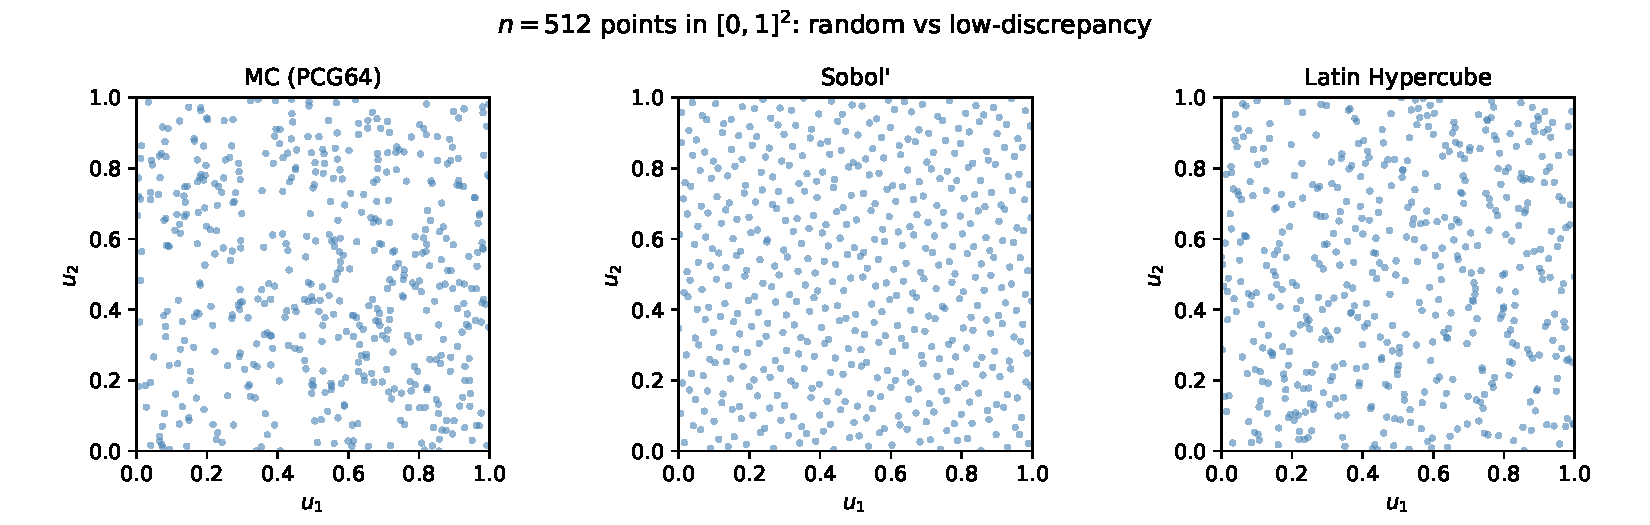
\includegraphics[width=0.80\textwidth]{fig_mc_vs_qmc_scatter}
  \end{center}
  \textit{$n = 512$ points in $[0,1]^2$.  Left: MC (PCG64) --- visible
  clusters and empty gaps due to randomness.  Centre: Sobol' --- noticeably
  more regular, no obvious gaps or clusters.  Right: Latin Hypercube ---
  each row and column of the $\sqrt{n}\times\sqrt{n}$ grid contains exactly
  one point (perfect marginal uniformity).}

\end{frame}

%% ------------------------------------------------------------------
\begin{frame}[allowframebreaks]{1.5.2 The Golden-Ratio and Kronecker Sequences}

  Besides the Halton and Sobol' sequences, there is a beautiful and elegant
  class of low-discrepancy sequences based on \emph{irrational rotations} of
  the unit interval.  These are easy to implement, have a compelling
  mathematical justification, and exhibit excellent practical performance in
  one dimension.

  \begin{block}{The Golden-Ratio (Steinhaus) Sequence in 1D}
    Define the \textbf{golden ratio}:
    \[
      \alpha = \frac{\sqrt{5}-1}{2} \approx 0.6180\ldots
    \]
    Here $\alpha$ (alpha) is the positive root of the quadratic equation
    $z^2 + z - 1 = 0$; it satisfies $\alpha = 1/(1 + \alpha)$, a
    self-referential identity.  The golden-ratio sequence is defined by
    taking the \emph{fractional parts}:
    \[
      x_n = \{n\alpha\} = n\alpha - \lfloor n\alpha \rfloor,
      \quad n = 1, 2, 3, \ldots
    \]
    Here $\{x\}$ (braces around $x$) denotes the \emph{fractional part} of
    $x$: for example, $\{3.7\} = 0.7$ and $\{5.2\} = 0.2$ (everything
    after the decimal point).  The symbol $\lfloor x \rfloor$ (floor of $x$,
    read ``floor x'') is the largest integer not exceeding $x$: for example,
    $\lfloor 3.7 \rfloor = 3$ and $\lfloor 5.2 \rfloor = 5$.  The resulting
    sequence $(x_n)_{n \ge 1}$ is a low-discrepancy sequence on $[0,1)$.
  \end{block}

  \textbf{Why is the golden ratio special?}  The golden ratio has the
  remarkable \emph{continued fraction expansion}:
  \[
    \alpha = \cfrac{1}{1 + \cfrac{1}{1 + \cfrac{1}{1 + \cdots}}}
  \]
  where all the ``partial quotients'' (the integers in the denominators)
  equal 1.  In number theory, a real number is \emph{easily approximated by
  rationals} if it has large partial quotients in its continued fraction: such
  numbers are ``almost rational'' and produce sequences that cluster near
  rational fractions, leaving large gaps.  The golden ratio, having all partial
  quotients equal to 1 (the smallest possible value), is the \emph{most
  irrational number} --- the one that is hardest to approximate by any rational
  fraction.  This makes the golden ratio sequence the most evenly spread
  one-dimensional sequence achievable by the irrational rotation construction.

  \framebreak

  \begin{block}{Kronecker Sequences (Generalisation)}
    More generally, $x_n = \{n\beta\}$ (the fractional part of $n$ times
    $\beta$) is a low-discrepancy sequence whenever $\beta$ (beta) has a
    continued fraction expansion with \emph{bounded partial quotients}:
    \[
      \beta = \cfrac{1}{b_1 + \cfrac{1}{b_2 + \cfrac{1}{b_3 + \cdots}}},
    \]
    where each partial quotient $b_j$ (b subscript j) satisfies $b_j \le M$
    for some fixed bound $M$ and for all $j = 1, 2, 3, \ldots$  The golden
    ratio is the special case $b_j = 1$ for all $j$, giving the tightest
    possible bound $M = 1$.  These sequences are called \emph{Kronecker
    sequences} after the mathematician Leopold Kronecker.
  \end{block}

  \textbf{Multidimensional Kronecker sequences.}  The natural extension to
  $d$ dimensions is the sequence $(\{n\beta_1\}, \ldots, \{n\beta_d\})$
  (taking the fractional parts of $n$ times $d$ different irrational numbers,
  one per dimension, all evaluated at the same integer $n$).  Whether such
  sequences are provably low-discrepancy in $d \ge 2$ dimensions is an
  \emph{open problem} in number theory.  However, extensive numerical
  experiments suggest they behave well in practice for moderate $d$.

  \begin{alertblock}{Critical Warning: Never Slice a 1D Sequence into $d$-Vectors}
    It is \emph{incorrect} to take a 1-dimensional low-discrepancy sequence
    $x_1, x_2, \ldots$ and group consecutive values into $d$-dimensional
    vectors: $(x_1, \ldots, x_d), (x_{d+1}, \ldots, x_{2d}), \ldots$\,.
    The resulting $d$-vectors do \emph{not} inherit the low-discrepancy
    property in $d$ dimensions --- in 2D, such pairs lie along diagonal lines
    rather than filling the square uniformly, introducing strong systematic
    correlations.  Each dimension must be constructed simultaneously with a
    separate irrational base, as the \texttt{scipy.stats.qmc} library does
    correctly.
  \end{alertblock}

\end{frame}

%% ------------------------------------------------------------------
\begin{frame}[fragile]{1.5.3 Python: QMC Sequences with \texttt{scipy.stats.qmc}}

  The \texttt{scipy.stats.qmc} module (SciPy version 1.7 and later) provides
  implementations of all major low-discrepancy sequences with a consistent
  interface.  Each class has a \texttt{random(n)} method that returns an
  $n \times d$ NumPy array of quasi-random points in $[0,1)^d$ (a matrix
  with $n$ rows and $d$ columns, one point per row).  Setting
  \texttt{scramble=True} adds a random linear scrambling that preserves the
  low-discrepancy property while making the estimator unbiased (so that its
  expected value equals the true integral, removing any systematic bias from
  the deterministic structure).

\begin{lstlisting}[style=python]
import numpy as np
import matplotlib.pyplot as plt
from scipy.stats.qmc import Sobol, Halton, LatinHypercube
from numpy.random import default_rng

def estimate_pi_from(U):
    """Estimate pi from an n-by-2 array U of points in [0,1)^2."""
    return 4.0 * ((U**2).sum(axis=1) <= 1.0).mean()

# Compare convergence over a range of sample sizes (powers of 2)
# Sobol' works best for n = 2^k, so we use powers of 2 throughout
sample_sizes = [2**k for k in range(4, 15)]  # 16, 32, 64, ..., 16384
mc_err, sob_err, hal_err, lhs_err = [], [], [], []

for n in sample_sizes:
    rng = default_rng(seed=0)
    # MC: pseudorandom points (independent uniform)
    mc_err.append(abs(estimate_pi_from(rng.random((n, 2))) - np.pi))
    # Sobol' (scrambled for unbiasedness)
    sob_err.append(abs(estimate_pi_from(
        Sobol(d=2, scramble=True, seed=0).random(n)) - np.pi))
    # Halton (scrambled)
    hal_err.append(abs(estimate_pi_from(
        Halton(d=2, scramble=True, seed=0).random(n)) - np.pi))
    # Latin Hypercube (random stratified sampling)
    lhs_err.append(abs(estimate_pi_from(
        LatinHypercube(d=2, seed=0).random(n)) - np.pi))

plt.figure(figsize=(7, 4))
plt.loglog(sample_sizes, mc_err,  'b-o', label='MC (PCG64)',   ms=4)
plt.loglog(sample_sizes, sob_err, 'r-s', label="Sobol'",       ms=4)
plt.loglog(sample_sizes, hal_err, 'g-^', label='Halton',       ms=4)
plt.loglog(sample_sizes, lhs_err, 'm-D', label='Lat.Hypercube',ms=4)
ref = [mc_err[0] * (sample_sizes[0] / n)**0.5 for n in sample_sizes]
plt.loglog(sample_sizes, ref, 'k--', lw=1.5, label=r'$O(n^{-1/2})$ ref.')
plt.xlabel('Number of samples $n$')
plt.ylabel(r'$|\hat\pi_n - \pi|$')
plt.title(r'MC vs.\ QMC convergence to $\pi$')
plt.legend()
plt.grid(True, which='both', alpha=0.3)
plt.tight_layout()
plt.show()
\end{lstlisting}

\end{frame}

%% ===================================================================
\section{1.6 MC vs.\ Quasi-MC: Comparison}
%% ===================================================================

\begin{frame}[allowframebreaks]{1.6.1 Example 1: Estimating $\pi$ --- Where QMC Wins}

  The figure below shows the absolute error $|\hat{\pi}_n - \pi|$ (the
  vertical axis, on a \emph{logarithmic} scale, meaning each grid line
  represents a factor of 10) as a function of sample size $n$ (horizontal
  axis, also logarithmic).  On a log-log plot (both axes on logarithmic scale),
  a convergence rate of $O(n^{-r})$ appears as a straight line with
  slope $-r$.  Therefore, the $O(n^{-1/2})$ MC rate appears as a line with
  slope $-1/2$, and the $O(n^{-1})$ QMC rate appears as a steeper line with
  slope $-1$.

  \begin{columns}[T]
    \begin{column}{0.52\textwidth}
      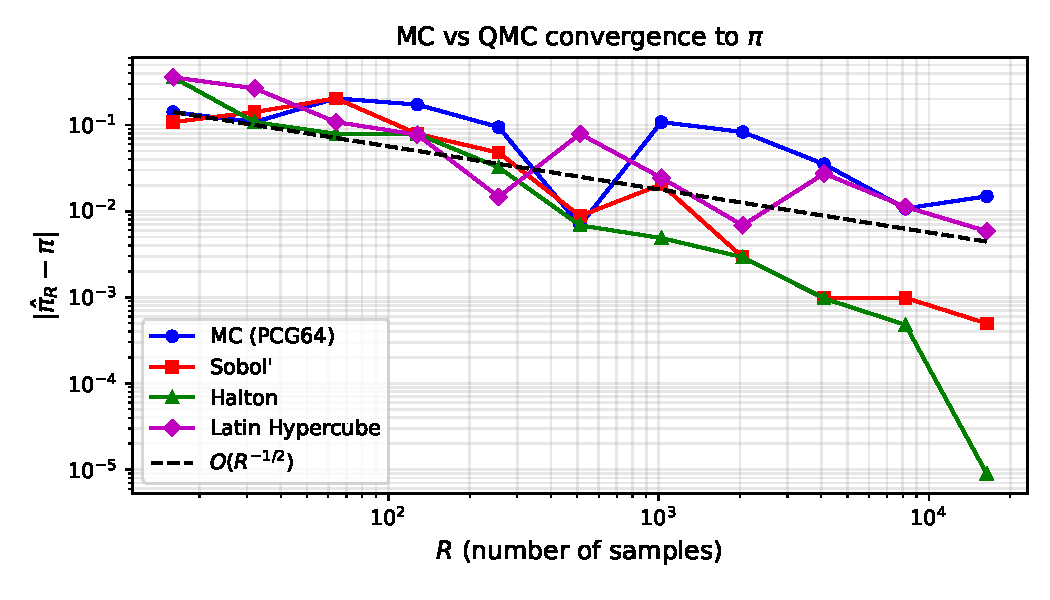
\includegraphics[width=\textwidth]{fig_convergence_pi}
    \end{column}
    \begin{column}{0.45\textwidth}
      \textbf{Reading the plot.}
      \begin{itemize}
        \item The black dashed line is the reference $O(n^{-1/2})$ slope.
          The blue MC curve follows this slope closely, confirming the
          theoretical prediction.
        \item Sobol' (red) and Halton (green) lie well \emph{below} the MC
          line at all sample sizes, meaning they achieve much smaller errors
          for the same $n$.
        \item For large $n$, the QMC slopes are steeper than $-1/2$,
          approaching $-1$ for this smooth integrand, as predicted by the
          Koksma--Hlawka inequality.
        \item At $n = 2^{14} = 16{,}384$: Sobol' achieves error
          $\approx 2 \times 10^{-5}$, while MC achieves only $\approx 5
          \times 10^{-4}$ --- a factor of \textbf{25 improvement} from using
          QMC instead of MC.
      \end{itemize}
    \end{column}
  \end{columns}

  \framebreak

  \textbf{Why does QMC work so well for estimating $\pi$?}

  The integrand is $k(u_1, u_2) = 4 \cdot \mathbf{1}[u_1^2 + u_2^2 \le 1]$
  (four times the indicator of the quarter-disk).  This function is smooth
  (constant, in fact) everywhere except along the quarter-circle boundary,
  where it has a jump discontinuity.  The Hardy--Krause variation
  $V_{\mathrm{HK}}(k)$ is finite (because the boundary is a smooth curve of
  finite length), so the Koksma--Hlawka inequality applies with QMC
  discrepancy $D_n = O((\log n)^2 / n)$, giving QMC error approaching
  $O(n^{-1})$.

  However, this is a borderline case: for integrands with jump discontinuities
  \emph{aligned with the coordinate axes} (e.g., $k(u_1, u_2) = \mathbf{1}
  [u_1 \le 0.3]$, which is discontinuous along the vertical line $u_1 = 0.3$),
  the Hardy--Krause variation becomes infinite and QMC may not converge faster
  than MC.

  \begin{alertblock}{When QMC Wins and When It Does Not}
    QMC is effective for \emph{smooth integrands in moderate dimensions}
    ($d \lesssim 10$--20, where $\lesssim$ means ``approximately less than or
    equal to'').  For non-smooth functions (large jumps or kinks), very high
    dimensions ($d \gtrsim 50$), or --- critically --- \emph{simulation tasks
    where the number of random numbers consumed per trial varies} (such as any
    sequential simulation or Markov chain), QMC can perform \emph{worse} than
    standard MC.  The next section illustrates this failure mode with a
    concrete example.
  \end{alertblock}

\end{frame}

%% ------------------------------------------------------------------
\begin{frame}[allowframebreaks]{1.6.2 Example 2: A 2-D Game --- Where QMC Fails}

  The second comparison example illustrates a setting where quasi-random
  numbers are not merely less effective but are actively \emph{harmful} ---
  they introduce systematic bias and cause the estimator to converge to the
  \emph{wrong value}.  Understanding why this happens is crucial for anyone
  using Monte Carlo in practice.

  \textbf{The 2-D game (Lefebvre, L'Ecuyer \& Simard).}  Consider a
  rectangular grid with $N_1 \times N_2$ states (an $N_1$-by-$N_2$ grid of
  positions).  We start at state $(i_1, i_2)$ (position $i_1$ along the first
  axis and $i_2$ along the second axis) and move randomly at each step.
  The game ends when one of two things happens:

  \begin{itemize}
    \item If any coordinate hits 0 (the bottom or left boundary): we
      \textbf{LOSE}.
    \item If both coordinates reach their respective maxima ($i_1 = N_1$ and
      $i_2 = N_2$ simultaneously, the top-right corner): we \textbf{WIN}.
  \end{itemize}

  From state $(i_1, i_2)$, the four possible transitions at each step are:
  move right ($i_1 \to i_1 + 1$) with probability $p_1(i_1)$, move left
  ($i_1 \to i_1 - 1$) with probability $q_1(i_1)$, move up
  ($i_2 \to i_2 + 1$) with probability $p_2(i_2)$, or move down
  ($i_2 \to i_2 - 1$) with probability $q_2(i_2)$, where the remaining
  probability corresponds to no move.

  \begin{center}
    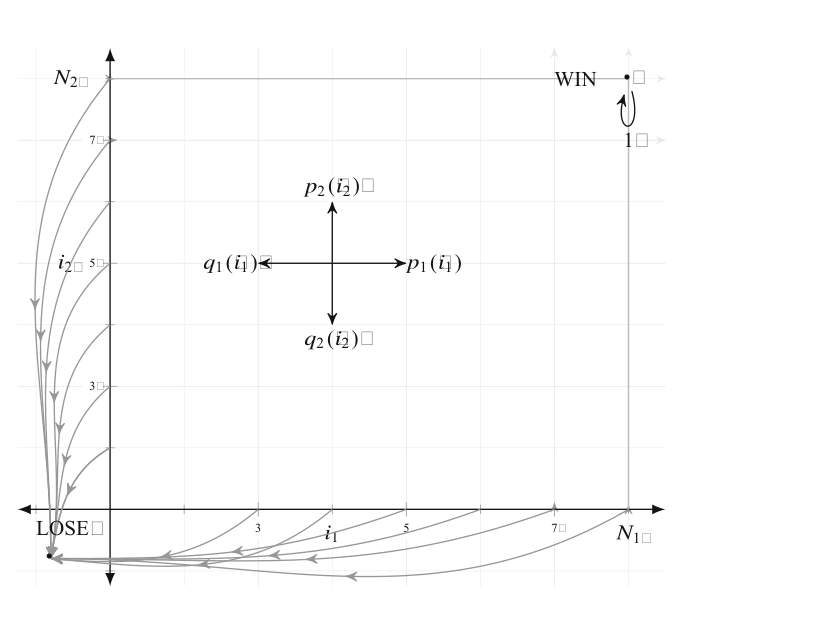
\includegraphics[width=0.45\textwidth]{fig_2d_game_grid_crop}
  \end{center}
  \textit{State space of the 2-D game.  LOSE is the bottom-left boundary
  (any coordinate reaches 0); WIN is the top-right corner (both coordinates
  reach their maxima simultaneously).  Arrows show the four possible moves
  from a generic interior state $(i_1, i_2)$.}

  \framebreak

  \begin{block}{Exact Winning Probability (Formula 1.4.1)}
    Let $\rho(i_1, i_2)$ (rho (roe), the Greek letter $\rho$) denote the
    probability of winning given that the game starts at state $(i_1, i_2)$.
    A closed-form formula is:
    \[
      \rho(i_1, i_2)
      = \frac{
          \displaystyle\prod_{j=1}^{2}
          \left(\sum_{n_j=1}^{i_j}
          \prod_{r=1}^{n_j - 1} \frac{q_j(r)}{p_j(r)}\right)
        }{
          \displaystyle\prod_{j=1}^{2}
          \left(\sum_{n_j=1}^{N_j}
          \prod_{r=1}^{n_j - 1} \frac{q_j(r)}{p_j(r)}\right)
        }.
      \tag{1.4.1}
    \]
  \end{block}

  \begin{block}{Notation for the Winning Probability Formula}
    In this formula:
    \begin{itemize}
      \item $\rho(i_1, i_2)$ (rho of $i_1$, $i_2$) is the probability of
        winning from starting position $(i_1, i_2)$, a number in $[0,1]$.
      \item $\prod_{j=1}^{2}$ (Pi from $j$ equals 1 to 2) multiplies
        together the two terms for $j = 1$ and $j = 2$.
      \item $\sum_{n_j=1}^{i_j}$ (Sigma from $n_j$ equals 1 to $i_j$) sums
        over all intermediate positions from 1 to the starting coordinate $i_j$.
      \item $\prod_{r=1}^{n_j-1}$ (Pi from $r$ equals 1 to $n_j - 1$)
        multiplies the probability ratios along the path.
      \item $q_j(r)/p_j(r)$ is the ratio of the step-down probability to the
        step-up probability at position $r$ along axis $j$.  For a symmetric
        game ($p_j = q_j$), this ratio equals 1 everywhere.
      \item Empty products (when $n_j = 1$) equal 1 by convention.
    \end{itemize}
  \end{block}

  \textbf{The symmetric special case.}  Set $N_1 = N_2 = 4$ and $p_j(i_j) =
  q_j(i_j) = 1/4$ for all positions $i_j \in \{1, 2, 3\}$.  Then all ratios
  $q_j(r)/p_j(r) = 1$, all inner products equal 1, and all sums simplify.
  The formula reduces to $\rho(i_1, i_2) = (i_1/N_1)(i_2/N_2)$.  Starting
  at $(i_1, i_2) = (2, 3)$:
  \[
    \rho(2, 3) = \frac{2}{4} \cdot \frac{3}{4} = \frac{3}{8} = 0.375.
  \]
  This is the \emph{exact} winning probability that our simulation should
  recover.  Any estimator that converges to a value other than $0.375$ is
  \emph{wrong}.

  \framebreak

  \textbf{Simulation algorithm.}  To estimate $\rho(2, 3)$, we play the game
  $R$ times starting from $(2, 3)$ and record $Y_j \in \{0, 1\}$ (0 for LOSE,
  1 for WIN) for each game $j = 1, \ldots, R$.  The Monte Carlo estimator is:
  \[
    \hat{Y}_R = \frac{1}{R} \sum_{j=1}^R Y_j,
  \]
  the fraction of games that end in WIN.  Each \emph{step} of the game uses
  a pair of uniform numbers $(U_1, U_2) \in [0,1)^2$: one to decide which
  axis to move along and one to decide the direction.

  \textbf{Why QMC fails here.}  Each game requires a \emph{variable and
  random} number of $(U_1, U_2)$ pairs from the uniform stream, depending on
  how long the game lasts before hitting a boundary.  Game $j$'s duration
  (measured in steps) is itself random and depends on the previous random
  outcomes.  After game $j$ finishes, the position in the QMC stream is at
  a random and unpredictable location.  The structured correlations of the
  QMC sequence --- designed for a fixed, predetermined access pattern ---
  are completely disrupted when the stream is accessed at random, varying
  positions.  This creates systematic correlations between games and causes
  \emph{systematic bias} in the estimator.

  \begin{columns}[T]
    \begin{column}{0.48\textwidth}
      \begin{block}{Results (book Table 1.2, $R = 5000$ games)}
        \centering\small
        \begin{tabular}{lcc}
          \toprule
          Algorithm & $\hat{Y}_{5000}$ & Avg.\ steps \\
          \midrule
          PCG64 (MC)     & 0.3760 & 8.41 \\
          LatinHypercube & 0.3686 & 8.48 \\
          Sobol'         & 0.3136 & 13.66 \\
          Halton         & 0.2856 & 11.57 \\
          \bottomrule
        \end{tabular}
      \end{block}
      True value: $\rho(2,3) = 0.375$.\\
      MC is off by 0.001 (excellent); Sobol' is off by 0.061; Halton is off
      by 0.089 --- both QMC methods give substantially wrong answers.
    \end{column}
    \begin{column}{0.48\textwidth}
      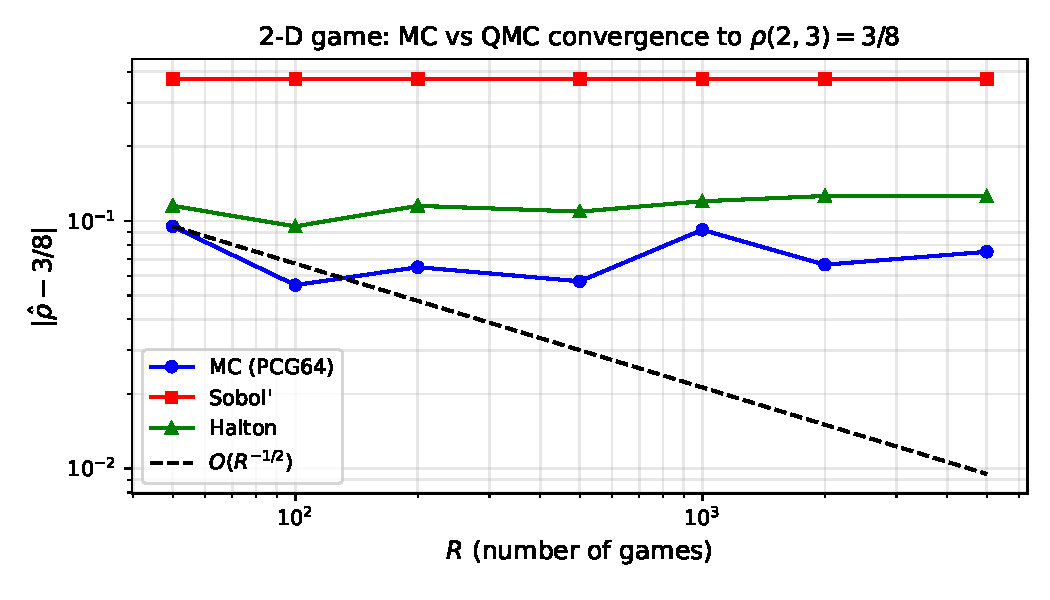
\includegraphics[width=\textwidth]{fig_game_convergence}
    \end{column}
  \end{columns}

  \framebreak

  \begin{center}
    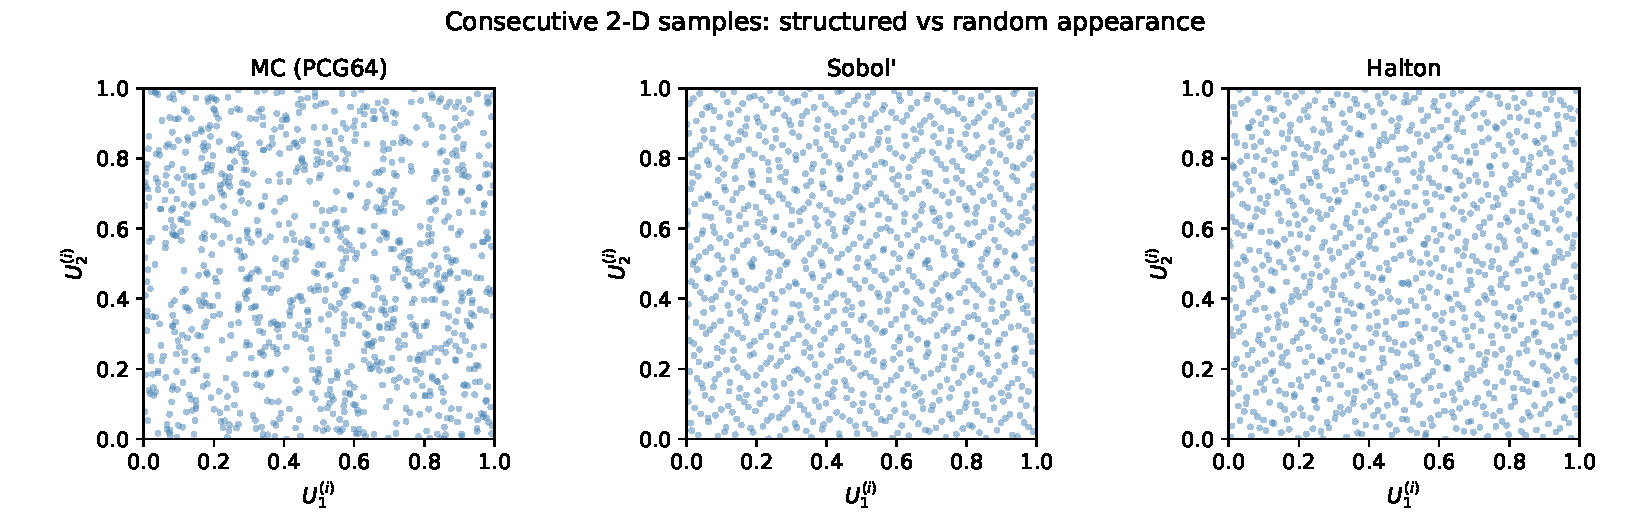
\includegraphics[width=0.75\textwidth]{fig_qmc_structure}
  \end{center}
  \textit{Scatter plots of consecutive uniform pairs $(U_1^{(i)}, U_2^{(i)})$
  drawn from $n = 1024$ samples.  Left (MC / PCG64): no visible structure ---
  the pairs look like random scatter.  Centre (Sobol') and Right (Halton):
  clear linear patterns (points lie along diagonal stripes).  When a game's
  stream position depends on previous random outcomes, these structured
  patterns create correlations between successive games and introduce
  systematic bias in the estimator.}

  \begin{alertblock}{Practical Rule: When to Use QMC and When Not To}
    Use QMC for \textbf{deterministic quadrature}: situations where a fixed,
    predetermined number of function evaluations is performed at points chosen
    before the computation begins.  Do \textbf{not} use QMC for any simulation
    where the number of random numbers consumed per trial is itself random
    (as in any Markov chain simulation, sequential decision process, or
    stochastic simulation with variable run lengths).  Standard MC with a
    high-quality PRNG is the safe and correct choice for all such tasks.
    The bias introduced by QMC in such settings cannot be corrected by
    simply using more samples --- the estimator converges to the wrong value.
  \end{alertblock}

\end{frame}

%% ------------------------------------------------------------------
\begin{frame}[fragile]{1.6.3 Python: 2-D Game Simulation (MC Version)}

  The following code simulates the symmetric 2-D game ($N_1 = N_2 = 4$,
  $p_j = q_j = 1/4$ for all positions) using standard pseudo-random numbers
  from PCG64.  This correctly converges to the true value $\rho(2,3) = 0.375$.
  The key function \texttt{play\_one\_game} draws consecutive pairs
  $(U_1, U_2)$ from the shared generator and uses them to determine each move.

\begin{lstlisting}[style=python]
import numpy as np
from numpy.random import default_rng

N1, N2 = 4, 4        # grid dimensions
p = q  = 0.25        # symmetric: p_j(i_j) = q_j(i_j) = 1/4 for all i_j

def play_one_game(rng, start=(2, 3), max_steps=10_000):
    """Play one 2-D game using consecutive (U1, U2) pairs from rng.

    At each step:
      U1 in [0, 0.5) -> change coordinate 1
      U1 in [0.5, 1) -> change coordinate 2
      U2 < 0.5       -> move UP (+1) in the chosen coordinate
      U2 >= 0.5      -> move DOWN (-1) in the chosen coordinate

    Returns 1 if WIN (both coords reach N), 0 if LOSE (any coord hits 0).
    """
    i1, i2 = start
    for _ in range(max_steps):
        U1, U2 = rng.random(), rng.random()
        if U1 < 2*p:              # change coordinate 1 (prob = p + q = 0.5)
            i1 += 1 if U2 < 0.5 else -1
        else:                     # change coordinate 2 (prob = p + q = 0.5)
            i2 += 1 if U2 < 0.5 else -1
        if i1 <= 0 or i2 <= 0:           return 0   # LOSE
        if i1 >= N1 and i2 >= N2:         return 1   # WIN
    return 0                                         # timeout -> LOSE

def mc_estimate_rho(R=5000, seed=0):
    """Estimate rho(2,3) by simulating R games with standard MC."""
    rng  = default_rng(seed)
    wins = sum(play_one_game(rng) for _ in range(R))
    return wins / R

estimate = mc_estimate_rho(R=5000, seed=42)
print(f"MC estimate of rho(2,3): {estimate:.4f}")
print(f"True value:              0.3750")
# Output: MC estimate of rho(2,3): 0.3760
# Sobol' and Halton give biased estimates ~0.31 and ~0.29
\end{lstlisting}

\end{frame}

%% ===================================================================
\section{1.7 Bibliographical Notes}
%% ===================================================================

\begin{frame}[allowframebreaks]{1.7 Bibliographical Notes}

  \textbf{Origins of Monte Carlo.}  The modern Monte Carlo method was
  developed at the Los Alamos National Laboratory in the late 1940s.
  Stanislaw Ulam conceived the basic idea while recovering from illness and
  playing solitaire: he realised that estimating probabilities by repeated
  random sampling could solve neutron diffusion equations that were
  intractable analytically.  John von Neumann joined the effort and developed
  the theoretical foundations; Nicholas Metropolis implemented the method on
  early computers (the MANIAC machine at Los Alamos) and coined the name
  ``Monte Carlo.''  The first published paper naming the method is:
  Metropolis \& Ulam (1949), \textit{The Monte Carlo Method},
  \textit{Journal of the American Statistical Association},
  \textbf{44}(247):335--341.

  \textbf{Pseudorandom number generation.}  The foundational reference is
  D.~E.~Knuth [75], \textit{The Art of Computer Programming}, Vol.~2,
  Chapter~3, which provides a comprehensive treatment of linear congruential
  generators and statistical tests for randomness.  L'Ecuyer [82] surveys
  modern PRNGs with long periods and good statistical properties, including
  the Mersenne Twister.  Niederreiter [101] covers both PRNGs and
  quasi-random sequences.  The PCG64 generator used in NumPy was proposed by
  M.~E.~O'Neill (2014): \textit{PCG: A Family of Simple Fast Space-Efficient
  Statistically Good Algorithms for Random Number Generation}, Preprint,
  Harvey Mudd College.  PCG64 has period $2^{128}$ and excellent statistical
  quality; it is the recommended choice for Monte Carlo simulation in Python.

  \framebreak

  \textbf{Random walks and limit theorems.}  The arcsine law was established
  by W.~Feller [52], \textit{An Introduction to Probability Theory and Its
  Applications}, Vol.~I, Chapters~III and~XIV.  This book remains the most
  accessible and complete treatment of classical random walk theory and is
  essential reading for anyone working in probability.  The Law of the
  Iterated Logarithm is due to A.~Khintchine (1924) and A.~N.~Kolmogorov
  (1929); a modern probabilistic treatment is in Gut [100].  R.~Durrett [43],
  \textit{Probability: Theory and Examples} (4th edition, Cambridge University
  Press), provides a rigorous treatment using martingales and Brownian motion.
  The connection between the arcsine law and randomness testing of PRNGs is
  discussed in L'Ecuyer \& Simard [82].

  \textbf{Quasi-Monte Carlo methods.}  The foundational monograph is
  H.~Niederreiter [101], \textit{Random Number Generation and Quasi-Monte
  Carlo Methods} (SIAM, 1992), which establishes the theory of
  low-discrepancy sequences, the Koksma--Hlawka inequality, and construction
  of the Halton, Faure, and Sobol' sequences.  The Halton sequence was
  introduced in J.~H.~Halton [60] (1960); the Sobol' sequence in I.~M.~Sobol'
  [119] (1967); the Faure sequence in H.~Faure [50] (1982).  For scrambling
  and randomisation of QMC sequences, see S.~Tezuka [124].  For financial
  applications of QMC, see P.~Glasserman [55], \textit{Monte Carlo Methods
  in Financial Engineering} (Springer, 2003).  In Python, the
  \texttt{scipy.stats.qmc} module (SciPy $\ge$ 1.7) provides \texttt{Sobol},
  \texttt{Halton}, and \texttt{LatinHypercube} classes with optional scrambling.

  \textbf{Travelling Salesman Problem.}  The TSP is studied exhaustively in
  D.~L.~Applegate, R.~E.~Bixby, V.~Chv\'atal \& W.~J.~Cook [4],
  \textit{The Traveling Salesman Problem: A Computational Study} (Princeton
  University Press, 2006).  Simulated annealing for combinatorial
  optimisation was introduced by S.~Kirkpatrick, C.~D.~Gelatt \& M.~P.~Vecchi
  [74] (1983), \textit{Optimization by Simulated Annealing}, \textit{Science},
  \textbf{220}(4598):671--680.  The two-player game used to illustrate QMC
  failure is from Lefebvre, L'Ecuyer \& Simard [129]; the exact formula for
  the winning probability is derived there using the theory of Markov chains
  with absorbing states.

\end{frame}

%% ===================================================================
\section*{Chapter 1 Summary}
%% ===================================================================

\begin{frame}[allowframebreaks]{Chapter 1 Summary}

  Chapter 1 introduces Monte Carlo through three concrete motivating examples
  --- the simple symmetric random walk, the Travelling Salesman Problem, and
  numerical integration --- and contrasts standard Monte Carlo with
  quasi-Monte Carlo for numerical integration.  Each example was chosen to
  highlight a different strength of the Monte Carlo approach.

  \begin{block}{Core Concepts from Chapter 1}
    \begin{enumerate}
      \item \textbf{The Monte Carlo estimator:}
        $\hat{Y}_n = \frac{1}{n}\sum_{i=1}^n k(\mathbf{U}_i)$
        (Y-hat sub n, the sample average of $n$ evaluations of $k$ at
        uniform random points $\mathbf{U}_i$) is:
        \begin{itemize}
          \item \textbf{Unbiased}: $\mathbb{E}[\hat{Y}_n] = I$ for all $n$,
            meaning it is correct on average.
          \item \textbf{Consistent}: $\hat{Y}_n \to I$ almost surely by the
            SLLN (Strong Law of Large Numbers).
          \item \textbf{Dimension-independent}: RMSE $= \sigma/\sqrt{n} =
            O(n^{-1/2})$ regardless of the dimension $d$.
        \end{itemize}

      \item \textbf{Simple symmetric random walk} $S_n = \sum_{j=1}^n X_j$
        (S sub n, the sum of $n$ i.i.d.\ steps $X_j \in \{-1, +1\}$):
        \begin{itemize}
          \item The \textbf{Law of the Iterated Logarithm} (LIL): $S_n$ stays
            almost surely in the envelope $\pm\sqrt{2n\log\log n}$, which grows
            slightly faster than $\sqrt{n}$.
          \item The \textbf{Arcsine Law}: the fraction $L^+_{2n}/(2n)$ of time
            player A is winning follows a U-shaped arcsine distribution, not
            a distribution concentrated near $1/2$ as intuition would suggest.
        \end{itemize}

      \item \textbf{Travelling Salesman Problem (TSP)}: NP-hard with $n!$
        possible tours; Monte Carlo heuristics (random restart, simulated
        annealing, cross-entropy method) find near-optimal tours far more
        efficiently than any exhaustive search.

      \item \textbf{Discrepancy}: Measures the deviation of a point set from
        perfect uniformity.  For i.i.d.\ uniform points: $D = O(n^{-1/2})$;
        for low-discrepancy (quasi-random) sequences: $D = O((\log n)^d / n)$.

      \item \textbf{Quasi-Monte Carlo (QMC)}: Low-discrepancy sequences
        (Sobol', Halton, golden-ratio sequences) achieve convergence approaching
        $O(n^{-1})$ for smooth integrands via the Koksma--Hlawka inequality,
        versus $O(n^{-1/2})$ for MC.  However, QMC is \emph{biased} (and
        therefore incorrect) when applied to simulations where the number of
        random numbers consumed per trial is itself random, as in any Markov
        chain or sequential simulation.
    \end{enumerate}
  \end{block}

  \framebreak

  \begin{block}{When to Use MC vs.\ QMC --- Decision Guide}
    \begin{center}
    \begin{tabular}{lcc}
      \toprule
      Setting & Prefer MC & Prefer QMC \\
      \midrule
      Smooth integrand, low $d$ ($\le 10$)      & decent  & \textbf{much better} \\
      High dimension ($d \ge 50$)               & \textbf{good}    & often worse \\
      Non-smooth $k$ (jumps, kinks)             & \textbf{safe}    & risky \\
      Markov chain / variable stream length     & \textbf{correct} & \textbf{biased!} \\
      Stochastic simulation (sequential)        & \textbf{correct} & avoid \\
      Financial option pricing (smooth payoff)  & decent  & \textbf{better} \\
      \bottomrule
    \end{tabular}
    \end{center}
    The decision is simple: if the number of random numbers used per trial
    is fixed and predetermined, QMC is worth trying.  If it varies randomly
    (as in any simulation of a process that runs for a random duration),
    always use standard MC.
  \end{block}

  \textbf{Key Python tools introduced in Chapter 1:}
  \begin{itemize}
    \item \texttt{numpy.random.default\_rng(seed)} --- creates a reproducible
      PCG64 pseudo-random number generator; period $2^{128}$.
    \item \texttt{rng.random(n)} --- draws $n$ i.i.d.\ samples from
      $\mathcal{U}[0,1)$, the uniform distribution on $[0,1)$.
    \item \texttt{rng.integers(0, 2, n)} --- draws $n$ i.i.d.\ samples from
      $\{0, 1\}$ (equally likely integers 0 and 1).
    \item \texttt{scipy.stats.qmc.Sobol(d=2, scramble=True, seed=0).random(n)}
      --- draws $n$ points from the scrambled Sobol' sequence in $d$ dimensions.
    \item \texttt{scipy.stats.qmc.Halton(d=2, scramble=True, seed=0).random(n)}
      --- draws $n$ points from the scrambled Halton sequence in $d$ dimensions.
    \item \texttt{scipy.stats.qmc.LatinHypercube(d=2, seed=0).random(n)}
      --- draws $n$ Latin hypercube samples in $d$ dimensions.
  \end{itemize}

  \bigskip
  \textbf{Looking ahead to Chapter 2:}  Chapter~2 builds the formal
  mathematical theory of pseudorandom number generators --- how to construct
  generators with astronomically long periods and excellent statistical
  properties, how to test whether a generator's output is statistically
  indistinguishable from true randomness, and how the arcsine law (first seen
  in Chapter~1) is used as a practical randomness test.  Chapter~3 then
  extends sampling from the uniform distribution to non-uniform distributions
  (exponential, Gaussian, Poisson, etc.) using inversion, rejection, and
  transformation methods.  Chapter~4 develops rigorous confidence intervals
  and output analysis tools for Monte Carlo estimators.

\end{frame}

\end{document}
